%%%%%%%%%%%%%%%%%%%%%%%%%%%%%%%%%%%%%%%%%%%%%%%%%%%%%%%%%%
%
% Doctoral Thesis Template @ The University of Manchester
% LaTeX Chapter Template
% Version 1 (23/07/2020)
% Joe Crone
%
% This template is based on:
% The University of Manchester, Presentation of Thesis Policy
% Research Office Graduate Education Team
% June 2017
% http://www.regulations.manchester.ac.uk/pgr-presentation-theses/
%
%%%%%%%%%%%%%%%%%%%%%%%%%%%%%%%%%%%%%%%%%%%%%%%%%%%%%%%%%%
\documentclass[../main.tex]{subfiles}
\begin{document}

% Title
%--------------------------------------------------------
\chapter{Optimisation and Characterisation of Inverse Compton Scattering Spectra}
\label{Optimisation_and_Characterisation_of_Inverse_Compton Scattering_Spectra} % to reference use \ref{ChapterTemplate}

\section{Motivation for Characterisation of ICS Sources}

Proper characterisation of inverse Compton scattering sources is necessary to quantify source performance and for reliable comparison between ICS sources. Through design and benchmarking of models used to predict ICS source performance and spectra, the ICS interactions of electron bunches and laser pulses can be better understood, which can reveal methods of improving narrowband ICS source design such as the optimisation strategies covered later in this chapter, which were motivated by the characterisation methods developed at the start of this chapter. The spectral output parameters presented in Chapter~\ref{Photon_Production_by_Inverse_Compton_Scattering}, such as flux and (average and peak) brilliance, fail to account for collimation effects, energy spread of the electron bunch and spectral bandwidth of the laser pulse. Therefore, models are required to predict the spectrum of the ICS source and quantify the affect of these parameters on the radiation spectrum available to the users of an ICS source. 

Within the first half of this chapter, an analytical approach to calculating the collimated flux produced by an ICS source is developed and compared to existing methods \cite{curatolo2017analytical} and a semi-analytical spectrum code \textsc{ICARUS}: inverse Compton scattering semi-analytical recoil-corrected ultra-relativistic spectrum code based on the model by Sun et al \cite{sun2009characterizations,sun2011theoretical}, which is corrected and expanded, is developed and benchmarked using the \textsc{ICCS3D} code \cite{krafft2016laser,ranjan2018simulation}. The characterisation methods developed here are tested through the use of three cases outlined in Section~\ref{sec:benchmarking_cases_characterisation_optimisation}, specified to cover the range of accelerators used to provide electron bunches to ICS sources; generalising the characterisation methods to any accelerator not just ERLs.

An analytical collimated flux equation has been developed in Section~\ref{sec:analytical_collimated_flux} in order to provide a quick, reliable method to predict the flux of an ICS source post-collimation with minimal assumptions. The analytical collimated flux calculation can also be used to predict the total photon yield (flux) of spectrum codes. Using the analytical method more accurate simulations such as those from spectrum codes can be evaluated. A wide variety of effects such as collimation, angular crossing and hourglass effects, described in Section~\ref{sec:geometric_luminosity_reduction}, have been incorporated into this methodology whilst the effect of energy spread of the electron bunch and spectral bandwidth of the laser pulse are notably neglected. Large-scale spectrum code simulations require computational time on the order of hours, with parallel computing whereas analytical calculations can be evaluated in sub-second timescales. Therefore, analytical collimated flux calculations are easier to apply to optimisation procedures rather than the more accurate spectral yield calculations from spectrum codes.   

The \textsc{ICARUS} spectrum code is a dedicated semi-analytical inverse Compton scattering code, which models the electron bunch--laser pulse interaction as Gaussian distributions and produces an ICS interaction spectrum
accounting for phenomena such as the recoil of the electron bunch, the emittance and divergence effects of the electron bunch and laser pulse and their energy spread and spectral bandwidth, as well as rectangular and circular collimation. However, the \textsc{ICARUS} spectrum code is limited to linear ICS interactions ($a_{0} \ll 1$) and head-on interactions ($\phi=0$). Methods have also been developed to calculate the collimated flux of an ICS source based upon these simulations. The \textsc{ICARUS} spectrum code is compared to two other ICS spectrum codes: Conglom\'{e}rat d'ABEL et d'Interactions Non-Lin\'{e}aires (\textsc{CAIN}) \cite{chen1995cain}, a Monte Carlo code for simulation of a broad range of electromagnetic interactions, and the Improved Codes for Compton Simulation (\textsc{ICCS3D}) \cite{krafft2016laser,ranjan2018simulation}, a semi-analytical code for simulation of ICS interactions. The comparison is detailed in Section~\ref{sec:} where spectrum simulation methods are discussed and the \textsc{ICARUS} code is benchmarked against the \textsc{ICCS3D} code.

\section{Analytical Collimated Flux}
\label{sec:analytical_collimated_flux}

In this section, the collimated flux - the total flux collected within an aperture of semi-angle $\theta_{\mathrm{col}}$ -- is derived from first principles, using the work of Berestetskii et al \cite{berestetskii1982quantum}. Unlike others in the literature \cite{curatolo2017analytical}, this method is valid for the angular crossing case ($\phi\in\mathbb{R}$) as the effect of the crossing angle is encompassed in the cross section as well as the geometric beam--beam angular crossing effect in Section~\ref{sec:geometric_luminosity_reduction}. The hourglass effect is also fully accounted for in this method, using the prescription of Miyahara \cite{miyahara2008luminosity}. The collimated flux calculation method is a semi-analytic calculation, requiring numerical integration, that is valid within the recoil regime (above $X\ll1$) but is only valid for the linear inverse Compton scattering case ($a_{0}\ll1$). The results of this derivation are benchmarked against a series of other methods including the the collimated flux formula by Curatolo et al \cite{curatolo2017analytical} and the \textsc{ICARUS} and \textsc{ICCS3D} spectrum codes in Section~\ref{sec:benchmarking_of_the_characterisation_methods}.

From previous derivations in Section~\ref{sec:electron_photon_interaction_cross_section}, the scattering angle $\theta$ dependence of the cross section (for example the differential cross section with respect to $Y$ (Eq.~\ref{eq:differential_cross_section_Y_invariant})) arises due to the the dependence of the scattering angle on the Lorentz invariant quantities $X$ (Eq.~\ref{eq:X_geometry}) and $Y$ (Eq.~\ref{eq:Y_geometry}) derived from Mandelstam variables in Section~\ref{sec:electron_photon_interactions}. Intrinsically, our definition of the recoil parameter $X$ (Eq.~\ref{eq:X_Mandelstam}) relates to the centre of mass $s$ Mandelstam variable before the interaction, so there is no scattering angle dependence as shown in (Eq.~\ref{eq:X_geometry}). However, the $Y$ Lorentx invariant is dependent on $\theta$, so this scattering angle dependence must be included via the derivative of $Y$ with $\theta$. Inspecting (Eq.~\ref{eq:Y_geometry}), we see $Y$ is dependent on $E_{\gamma}$, the scattered photon energy (Eq.~\ref{eq:scattered_photon_energy}) derived in Section~\ref{sec:derivation_of_the_scattered_photon_energy}, which also depends on scattering angle. Expansion of $Y$ in terms of the scattered photon energy scattering angle dependence is necessary, which can be simplified in terms of the recoil parameter $X$ (Eq.~\ref{eq:X_geometry}),
\begin{equation}
Y = \frac{2\gamma E_{L}\left(1+\beta\cos\phi\right)\left(1-\beta\cos\theta\right)}{m_{e}c^{2}\left\{1-\beta\cos\theta+\left[1+\cos\left(\phi+\theta\right)\right]E_{L}/E_{e}\right\}} = \frac{X\left(1-\beta\cos\theta\right)}{1-\beta\cos\theta+\left[1+\cos\left(\phi+\theta\right)\right]E_{L}/E_{e}}.
\label{eq:Y_geometry_expanded}
\end{equation}
The derivative of the expanded $Y$ Lorentz invariant (Eq.~\ref{eq:Y_geometry_expanded}) is then found using the quotient rule and the full derivative of $Y$ by $\theta$ becomes
\begin{equation}
\frac{dY}{d\theta} = \frac{X\beta\sin\theta\zeta-X\left(1-\beta\cos\theta\right)\left[\beta\sin\theta-\sin\left(\phi+\theta\right)E_{L}/E_{e}\right]}{\zeta^{2}}.
\label{eq:dY_dtheta}
\end{equation}
which is simplified using
\begin{equation}
\zeta = 1-\beta\cos\theta+\left[1+\cos\left(\phi+\theta\right)\right]E_{L}/E_{e}
\label{eq:zeta_simplification}
\end{equation}

Following the description of the interaction in Section~\ref{sec:electron_photon_interaction_cross_section}, and the subsequent derivation the differential cross section in with respect to the $Y$ Lorentz invariant in (Eq.~\ref{eq:differential_cross_section_Y_invariant}) is given by 
\begin{equation*}
\frac{d\sigma}{dY} = \frac{8\pi r_{e}^{2}}{X^{2}}\left\{\left[\left(\frac{1}{X}-\frac{1}{Y}\right)^{2}+\frac{1}{X}-\frac{1}{Y}\right]+\frac{1}{4}\left(\frac{X}{Y}+\frac{Y}{X}\right)\right\}.
\end{equation*}
To recap the derivation of (Eq.~\ref{eq:differential_cross_section_Y_invariant}) in Section~\ref{sec:electron_photon_interaction_cross_section}, we assume ambivalence over the polarisation states of the scattered photons in the double differential cross section (Eq.~\ref{eq:polarisation_differential_cross_section}) -- no single polarisation state or direction is selected -- yielding (Eq.~\ref{eq:double_differential_cross_section}), with dependence on the incident photon polarisation state. As all photons produced from any azimuthal scattering angle $\phi_{f}$ are collected, the full range ($0 \leq \phi_{f} \leq 2\pi$) is integrated and the differential cross section with respect to $Y$ becomes that given in (Eq.~\ref{eq:differential_cross_section_Y_invariant}). Integration over the azimuthal scattering angle removes the incident photon polarisation dependence, therefore the differential cross section (Eq.~\ref{eq:differential_cross_section_Y_invariant}), and consequently the collimated flux, are independent of initial and scattered photon polarisations.

The dependence of the cross section $\sigma$ on the scattering angle $\theta$ is then given by the chain rule
\begin{equation}
\frac{d\sigma}{d\theta} = \frac{d\sigma}{dY}\frac{dY}{d\theta},
\label{eq:cross_section_chain_rule}
\end{equation}
therefore the cross section for a collimation angle $\theta_{\mathrm{col}}$ becomes
\begin{equation}
\sigma\left(\theta_{\mathrm{col}}\right) = \int_{0}^{\theta_{\mathrm{col}}}\frac{d\sigma}{dY}\frac{dY}{d\theta}d\theta,
\label{eq:cross_section_integral}
\end{equation} 
where $d\sigma/dY$ is given by (Eq.~\ref{eq:differential_cross_section_Y_invariant}) and $dY/d\theta$ is given by (Eq.~\ref{eq:dY_dtheta}). The derivation of the recoil parameter (Eq.~\ref{eq:X_geometry}) accounts for the crossing angle between the incident photon and the incident electron, therefore this cross section is fully generalised for any interaction geometry.

Using the result derived in Section~\ref{sec:luminosity_and_flux}, the collimated flux is given by a modified form of the flux equation (Eq.~\ref{eq:headon_flux}), where the cross section (Eq.~\ref{eq:full_scattering_angle_cross_section_integral}) is replaced by the scattering angle dependent cross section (Eq.~\ref{eq:cross_section_integral}). The geometric luminosity angular crossing and the  hourglass effect, as explained in Section~\ref{sec:geometric_luminosity_reduction}, are accounted for using (Eq.~\ref{eq:miyahara_combined_reduction}) by Miyahara \cite{miyahara2008luminosity} which generalises the collimated flux for any electron bunch--laser pulse interaction geometry. Similarly to  the uncollimated flux (Eq.~\ref{eq:flux_angular_crossing_hourglass}), the collimated flux becomes
\begin{equation}
\mathcal{F}_{\mathrm{col}} = \sigma\left(\theta_{\mathrm{col}}\right) R_{ACHG}\mathcal{L}_{\mathrm{HEAD-ON}}f.
\label{eq:collimated_flux}
\end{equation}

It is inherent in (Eq.~\ref{eq:collimated_flux}) that the interaction occurs from a point source -- the transverse and longitudinal positions of the electrons within the bunch are neglected. However, as explained in Section~\ref{sec:source_size_divergence}, the point source approximation is valid whilst the transverse (longitudinal) source size is much smaller than the collimator aperture radius (source-to-collimator distance) -- termed far-field collimation. Within (Eq.~\ref{eq:collimated_flux}) the effect of the energy spread of the electron bunch, the spectral bandwidth and partially, via the point source approximation, the effect of the emittance (spatial extent) of the bunch are neglected. The codes \textsc{ICARUS} and \textsc{ICCS3D} \cite{krafft2016laser,ranjan2018simulation} properly take into account the energy spread factors but the emission position problem is only solved in Monte Carlo codes such as \texsc{CAIN} \cite{chen1995cain}. However, this effect is expected to be small as most ICS sources use far-field collimation.

\section{Development of the ICARUS Spectrum code}
\label{sec:development_of_the_ICARUS_spectrum_code}

\textsc{ICARUS}: inverse Compton scattering semi-analytic recoil-corrected ultra-relativistic spectrum code, uses a modified (and corrected) version of the 2D ICS spectrum model created by Sun et al. \cite{sun2009characterizations,sun2011theoretical} to generate the spectrum of radiation produced by an ICS source. The \textsc{ICARUS} code is valid for large electron recoil ($X\sim1$) and the linear regime ($a_{0}\ll 1$). \textsc{ICARUS} calculates the number of photons produced at small energy intervals that pass through a given far-field collimator aperture (circular or rectangular) for the fundamental laser mode. The simulated radiation spectrum is that observable at a detector placed downstream of a collimator. \textsc{ICARUS} assumes that the electron bunch and laser pulse are modelled by 3D Gaussian distributions, and can account for both circularly and linearly polarised incident photons. However, \textsc{ICARUS} is currently only valid for the head-on ($\phi = 0$) geometry.

Using the result of Sun et al \cite{sun2009characterizations,sun2011theoretical}, the distribution of a $\gamma$-ray beam produced by a head-on collision of an electron bunch and laser pulse is given by
\begin{multline}
\frac{dN_{\gamma}}{d\Omega_{c} dE_{\gamma}} = N_{e}N_{L}\int \frac{d\sigma}{d\Omega}\delta\left(\bar{E_{\gamma}}-E_{\gamma}\right)c\left(1+\beta\right)f_{e}\left(x,y,z,x',y',p,t\right)\\ \times f_L\left(x,y,z,k,t\right)dx'~dy'~dp~dk~dV~dt,
\label{eq:central_distribution_sun}
\end{multline}
where the collimator solid angle is $d\Omega_{c} = dx_{c}dy_{c}/L^{2}$ with $x_{c}$ and $y_{c}$ the $x$ and $y$ positions at the collimator and $L$ the source-to-collimator distance, $d\sigma/d\Omega$ is the differential cross section of the ICS interaction, $\delta\left(\bar{E_{\gamma}}-E_{\gamma}\right)$ is a delta function which encapsulates energy conservation in the process with $\bar{E_{\gamma}}$ the maximum possible energy a $\gamma$-ray have for a scattering angle $\theta$ and $E_{\gamma}$ the actual $\gamma$-ray energy, the $c\left(1+\beta\right)$ term arises from the Doppler shifting of the radiation, $f_{e}$ and $f_{L}$ are the phase-space intensity distributions of the electron bunch (Eq.~\ref{eq:electron_gaussian_intensity_distribution}) and laser pulse (Eq.~\ref{eq:laser_gaussian_intensity_distribution}) as modelled by Gaussian distributions, $dx'$ and $dy'$ are the divergence integration variables in $x$ and $y$ respectively, $dp$ is momentum of the electron integration variable, $dk$ is the wavenumber of the laser pulse integration variable, $dV$ is the volume of the interaction integration parameter and  $dt$ is the interaction time integration variable. 

The differential cross section for a head-on ($\phi=0$) collision in this model is given by
\begin{equation}
\frac{d\sigma}{d\Omega} = 8\pi r_{e}^{2}\left\{\frac{1}{4}\left[\frac{4\gamma^{2}E_{L}}{\bar{E_{\gamma}}\left(1+\gamma^{2}\theta^{2}\right)}+\frac{\bar{E_{\gamma}}\left(1+\gamma^{2}\theta^{2}\right)}{4\gamma^{2}E_{\gamma}}\right]-2\cos^{2}\left(\tau-\phi_{f}\right)\frac{\gamma^{2}\theta^{2}}{\left(1+\gamma^{2}\theta^{2}\right)^{2}}\right\}\left(\frac{\bar{E_{\gamma}}}{4\gamma E_{L}}\right)^{2},
\label{eq:sun_differential_cross_section}    
\end{equation}
where $\bar{E_{\gamma}}$ is the scattered photon energy for a particular scattering angle $\theta$ in the small angle approximation for a head-on ($\phi=0$) collision
\begin{equation}
\bar{E_{\gamma}} = \frac{4\gamma^{2}E_{L}}{1+\gamma^{2}\theta^{2}+\frac{4\gamma E_{L}}{m_{e}c^{2}}}.
\label{eq:sun_Egamma_bar}    
\end{equation}
The angular divergences of the scattered photons $x'$ and $y'$ can be expressed the projection of the scattering angle of of the produced radiation in each plane $\theta_{x}'$ and $\theta_{y}'$ ($\theta = \sqrt{\theta_{x}^{2}+\theta_{y}^{2}}$) using the relations
\begin{align}
\theta_{x}' + x' &= \frac{x_{c}-x}{L}, & \theta_{y}' + y' &= \frac{y_{c}-y}{L}
\label{eq:sun_angular_divergence}    
\end{align}
which arise from the geometric constraints of a photon passing through a collimator and then impinging on a detector in far-field collimation ($L \gg \sqrt{x_{c}^{2}+y_{c}^{2}}$), where $x$ and $y$ are the positions of the scattered photon on the collimator aperture in each direction. Here the small angular divergences of the laser pulse have been neglected. The model can be simply extended for collimator misalignment, through addition of a simple error term \cite{sun2009characterizations} $x_{\mathrm{err}}$ or $y_{\mathrm{err}}$, where the angular divergences become
\begin{align}
\theta_{x}' + x' &= \frac{x_{c}-x-x_{\mathrm{err}}}{L}, &
\theta_{y}' + y' &= \frac{y_{c}-y-y_{\mathrm{err}}}{L}
\label{eq:sun_collimator_misallignment}    
\end{align}

Applying (Eq.~\ref{eq:sun_angular_divergence}) and integrating (Eq.~\ref{eq:central_distribution_sun}) with respect to $dV$, the interaction volume, and $dt$ the interaction time, whilst expanding the detector solid angle, the Gaussian intensity distributions of the electron bunch (Eq.~\ref{eq:electron_gaussian_intensity_distribution}) and laser pulse (Eq.~\ref{eq:laser_gaussian_intensity_distribution}), yields
\begin{multline}
\frac{dN_{\gamma}}{dE_{\gamma}dx_{c}dy_{c}} = \frac{N_{e}N_{L}}{\left(2\pi\right)^{3}z_{R}\sigma_{p}\sigma_{k}}\int \frac{k}{\sqrt{\zeta_{x}\zeta_{y}}\sigma_{\theta_{x}}\sigma_{\theta_{y}}}\frac{d\sigma}{d\Omega}\delta\left(\bar{E_{\gamma}}-E_{\gamma}\right)\left(1+\beta\right) \\\times\exp\left[-\frac{\left(\theta_{x}-x_{c}/L\right)^{2}}{2\sigma_{\theta_{x}}^{2}}-\frac{\left(\theta_{y}-y_{c}/L\right)^{2}}{2\sigma_{\theta_{y}}^{2}}-\frac{\left(p-p_{0}\right)^{2}}{2\sigma_{p}^{2}}-\frac{\left(k-k_{0}\right)^{2}}{2\sigma_{k}^{2}}\right]~d\theta_{x}~d\theta_{y}~dp~dk,
\label{eq:sun_volume_time_integral}    
\end{multline}
where $z_{R}$ is the Rayleigh range (Eq.~\ref{eq:rayleigh_range}), and the $\zeta_{x/y}$, $\sigma_{\theta_{x/y}}$ and $\xi_{x/y}$ parameters in each plane are given by
\begin{align}
\zeta_{x} &= 1+\frac{2k\beta_{x}\epsilon_{x}}{z_{R}}, & \sigma_{\theta_{x}} &= \sqrt{\frac{\epsilon_{x}\xi_{x}}{\beta_{x}\zeta_{x}}}, & \xi_{x} &= 1+\left(\alpha_{x}-\frac{\beta_{x}}{L}\right)^{2}+\frac{2k\beta_{x}\epsilon_{x}}{z_{R}}, \nonumber\\
\zeta_{y} &= 1+\frac{2k\beta_{y}\epsilon_{y}}{z_{R}}, & \sigma_{\theta_{y}} &= \sqrt{\frac{\epsilon_{y}\xi_{y}}{\beta_{y}\zeta_{y}}}, & \xi_{y} &= 1+\left(\alpha_{y}-\frac{\beta_{y}}{L}\right)^{2}+\frac{2k\beta_{y}\epsilon_{y}}{z_{R}}, 
\label{eq:zeta_sigmatheta_xi_parameters_sun}
\end{align}
where $p_{0}$ is the reference momentum of the electron bunch and $k_{0}$ is the centroid wavenumber of the laser pulse (the wavenumber of the fundamental harmonic). Note that there is an algebraic error in Sun et al's \cite{sun2009characterizations,sun2011theoretical} derivation; Sun et al's pre-factor states that $dN/dE\propto L^{2}$ for a source-to-collimator distance $L$. The error occurs because of a mishandling of the detector solid angle. Clearly, this should be $dN/dE\propto 1/L^{2}$, meaning there is an inverse square relationship between source-to-collimator distance and the spectral density and this is corrected within the \textsc{ICARUS} code. 

The delta function, encompassing the energy conservation of the interaction, can be re-wrote in terms of the Lorentz factor
\begin{equation}
\delta\left(\bar{E_{\gamma}}-E_{\gamma}\right) = -\delta\left(\gamma-\bar{\gamma}\right)\frac{\left(1+\bar{\gamma}^{2}\theta^{2}+\frac{4\bar{\gamma}E_{L}}{m_{e}c^{2}}\right)^{2}}{8\bar{\gamma}E_{L}\left(1+\frac{2\bar{\gamma}E_{L}}{m_{e}c^{2}}\right)},
\label{eq:sun_electron_energy_delta_function}    
\end{equation}
where $\bar{\gamma}$ is the root of $\bar{E_{\gamma}}$ (Eq.~\ref{eq:sun_Egamma_bar}) as given by
\begin{equation}
\bar{\gamma} = \frac{2E_{\gamma}E_{L}}{m_{e}c^{2}\left(4E_{L}-E_{\gamma}\theta^{2}\right)}\left[1+\sqrt{1+\frac{4E_{L}-E_{\gamma}\theta^{2}}{4E_{L}^{2}E_{\gamma}/\left(m_{e}c^{2}\right)^{2}}}\right].    
\end{equation}

Substituting for $\delta\left(\bar{E_{\gamma}-E_{\gamma}}\right)$ using (Eq.~\ref{eq:sun_electron_energy_delta_function}) and simply exchanging the electron bunch momentum variable from $dp$ to $d\gamma$, (Eq.~\ref{eq:sun_volume_time_integral}) is integrated with respect to $d\gamma$ to introduce the electron bunch energy spread variation, which becomes
\begin{multline}
\frac{dN_{\gamma}}{dE_{\gamma}} = \frac{r_{e}^{2}N_{e}N_{L}}{4\pi^{3}L^{2}\hbar c z_{R}\sigma_{\gamma}\sigma_{k}}\int_{k_{\mathrm{min}}}^{k_{\mathrm{max}}}\int_{-\theta_{x,\mathrm{max}}}^{\theta_{x,\mathrm{max}}}\int_{-\theta_{y,\mathrm{max}}}^{\theta_{y,\mathrm{max}}}\int_{y_{\mathrm{min}}}^{y_{\mathrm{max}}}\int_{x_{\mathrm{min}}}^{x_{\mathrm{max}}}\frac{1}{\sqrt{\zeta_{x}\zeta_{y}}\sigma_{\theta_{x}}\sigma_{\theta_{y}}}\frac{\bar{\gamma}}{1+2\gamma E_{L}/m_{e}c^{2}} \\
\times\left\{\frac{1}{4}\left[\frac{4\bar{\gamma}^{2}E_{L}}{E_{\gamma}\left(1+\bar{\gamma}^{2}\theta^{2}\right)}+\frac{E_{\gamma}\left(1+\bar{\gamma}^{2}\theta^{2}\right)}{4\bar{\gamma}^{2}E_{L}}\right]-2\cos^{2}\left(\tau-\phi_{f}\right)\frac{\bar{\gamma}^{2}\theta^{2}}{\left(1+\bar{\gamma}^{2}\theta^{2}\right)^{2}}\right\} \\
\times\exp{\left[-\frac{\left(\theta_{x}-x_{c}/L\right)^{2}}{2\sigma_{\theta_{x}}^{2}}-\frac{\left(\theta_{y}-y_{c}/L\right)^{2}}{2\sigma_{\theta_{y}}^{2}}-\frac{\left(\gamma-\gamma_{0}\right)^{2}}{2\sigma_{\gamma}^{2}}-\frac{\left(k-k_{0}\right)^{2}}{2\sigma_{k}^{2}}\right]}dx_{c}~dy_{c}~d\theta_{y}~d\theta_{x}~dk,
\label{eq:ICARUS_equation}
\end{multline}
where the cross section has been expanded in terms of the $\bar{\gamma}$ parameter with a normalisation factor in the third term, $\gamma_{0}$ is the centroid Lorentz factor of the electron bunch, $\sigma_{\gamma} = \sigma_{e}/m_{e}c^{2}$ is the spread of the Lorentz factor of the electron bunch. Integral limits have been imposed on each of the integrations, as discussed below. 

The integral over the horizontal collimator aperture $dx_{c}$ (vertical collimator aperture $dy_{c}$) can be carried out with the limits $x_{\mathrm{min}}$ and $x_{\mathrm{max}}$ ($y_{\mathrm{min}}$ and $y_{\mathrm{max}}$), which vary dependent on the collimator shape (rectangular or circular) and based on the specified collimator dimensions. For the circular collimation case, the relationship $R\geq\sqrt{x_{c}^{2}+y_{c}^{2}}$ must be obeyed with $R$ the radius of the collimator. For example, in the horizontal $x$ plane $x_{\mathrm{min}} = -R$ and $x_{\mathrm{max}} = R$, such that the limits are equal to the radius of the collimator. However this means that in the $y$ plane, the collimator position integration limits are a function of $x_{c}$: $y_{\mathrm{min}} = -\sqrt{R^{2}-x_{c}^{2}}$ and $y_{\mathrm{max}} = \sqrt{R^{2}-x_{c}^{2}}$. For the case of a rectangular collimator these limits can be treated independently.  
Integrals over the projection of the scattering angles in each plane are carried out using the limits
\begin{align}
\theta_{x,\mathrm{max}} &= \sqrt{\frac{4E_{L}}{E_{\gamma}}-\theta_{y}^{2}}, & \theta_{x,\mathrm{min}} &= -\sqrt{\frac{4E_{L}}{E_{\gamma}}-\theta_{y}^{2}} \nonumber\\ 
\theta_{y,\mathrm{max}} &= \sqrt{\frac{4E_{L}}{E_{\gamma}}}, & \theta_{y,\mathrm{min}} &= -\sqrt{\frac{4E_{L}}{E_{\gamma}}},  
\end{align}
which constrains the angular cone the radiation is produced into to a maximum of a $1/\gamma$ cone in two dimensions -- the collimation angle typically limits $E_{\gamma}$ so that the cone is smaller than $1/\gamma$. As the limits of the $\theta_{x}$ integral are dependent on $\theta_{y}$, the order of integration is constrained and $\theta_{y}$ must be evaluated before $\theta_{x}$. The order of integration is similarly constrained for the integration over a circular collimator aperture -- $x_{c}$ must be integrated before $y_{c}$.

The wavenumber $k$ of the incident laser photon in Sun et al's model \cite{sun2009characterizations,sun2011theoretical} is integrated from $0$ to $\infty$, to reflect a summation over all possible laser harmonics. However, this is impractical in a real simulation and unnecessary for laser driven sources because the fundamental harmonic is the laser wavelength of interest and other harmonics will have a negligibly weak contribution to the spectra for $a_{0} \ll 1$ or be excluded completely due to re-circulation in a Fabry-Perot optical cavity. Therefore, the limit for the integration of the wavenumber of the incident laser is set to $k\pm3\sigma_{k}$, representing the 3$\sigma_{k}$ spectral bandwidth tail of the laser pulse, as the laser pulse is modelled using a Gaussian distribution.  

The polarisation term $2\cos^{2}\left(\tau-\phi_{f}\right)$ in (Eq.~\ref{eq:ICARUS_equation}) must be modified as the azimuthal scattering angle $\phi_{f}$ is not explicitly integrated, instead the azimuthal scattering angle dependence is incorporated into the integration of the projection of the scattering angles ($\theta_{x}$ and $\theta_{y}$) in each plane. Therefore, the azimuthal scattering angle $\phi_{f}$ in (Eq.~\ref{eq:ICARUS_equation}) is replaced by $\phi_{f} = \cos^{-1}\left(\theta_{x}/\theta\right)$. The $x$ plane projection of the scattering angle $\theta_{x}$ is selected over the $y$ plane due to order of integration constraints. However, when integrated over the full azimuthal scattering angle ($0 \leq \phi_{f} \leq 2\pi$) -- which occurs during the spectrum code simulation -- the polarisation term has no effect, as expected.

The \textsc{ICARUS} spectrum code functions as a \textsc{Mathematica} script with pre-input of ICS source parameters (electron bunch and laser pulse parameters), often from the optimisations later in this chapter, and post-processing which produces plots of spectra from the developed model and calculates the spectral yield (collimated flux) from the produced spectrum. The spectral yield (collimated flux) is calculated by 
\begin{equation}
\mathcal{F}_{\mathrm{col}} = R_{AC}f\mathcal{F}^{\mathrm{spec}}_{\mathrm{col}}    
\label{eq:spectral_yield}
\end{equation}
where $R_{AC}$ is the crossing angle luminosity reduction factor (Eq.~\ref{eq:angular_crossing_factor}), which adjusts the head-on spectrum flux for the crossing angle of the interaction because \textsc{ICARUS} only simulates head-on interactions, $f$ is the repetition rate of interactions of the source, included because the \textsc{ICARUS} simulation only simulates a single electron bunch--laser pulse interaction and $\mathcal{F}^{\mathrm{spec}}_{\mathrm{col}}$ is the spectral yield (collimated flux) of a single electron bunch--laser pulse interaction -- the area under the \textsc{ICARUS} spectrum. The spectral yield can be applied more generally to calculate the collimated flux from any spectrum code. 

The \textsc{ICARUS} simulation evaluates (Eq.~\ref{eq:ICARUS_equation}) at a series of scattered photon energy points to determine the number of photons produced at scattered photon energy intervals thereby building up a spectrum. The maximum scattered photon energy to sample for the spectrum calculation is calculated using (Eq.~\ref{eq:scattered_photon_energy}) with $E_{e}+3\sigma_{e}$ as the electron bunch energy because of the Gaussian distribution of electron energies. with non-negligible energy spread. However, this neglects the laser pulse spectral bandwidth because the electron bunch energy has a squared dependence on scattered photon energy ($E_{\gamma}\propto\gamma^{2}$), in comparison to scattered photon energies linear relationship with laser pulse energy, therefore it is a reasonable to neglect the spectral bandwidth of the laser pulse unless the spectral bandwidth of the laser is large. The minimum sampled scattered photon energy is approximated as
\begin{equation}
E_{\gamma,\mathrm{min}} \approx E_{\gamma}\left[1-3\left(\frac{\Delta E_{\gamma}}{E_{\gamma}}\right)_{\mathrm{FWHM}}\right],
\label{eq:ICARUS_minimum_energy}
\end{equation}
where the Compton edge energy reduced by a factor of $3\sigma$, with sigma the full-width half-maximum bandwidth (Eq.~\ref{eq:FWHM_bandwidth}) of the ICS source being simulated. The minimum energy is generally appropriate for ICS spectra, however when the spectrum is highly dominated by strong collimation $E_{\gamma,\mathrm{min}}$ is much smaller than the scattered photon energy of the low energy tail of the spectrum. One hundred points in the scattered photon energy range are typically calculated, but the number of simulation points is determined due to the computational time and precision requirements of the user -- simulation time typically scales linearly with simulation points.  

For the complex integration involved in evaluating the central equation of \textsc{ICARUS} (Eq.~\ref{eq:ICARUS_equation}), quasi-Monte Carlo (QMC) integration methods are used alongside parallel-processing, where each node calculates an individual scattered photon energy point in the simulation. Typically 100 million QMC points are used to create a precise spectrum, though this simulation parameter can be adjusted with greater precision (more QMC points) with greater simulation time. The Gaussian functions in (Eq.~\ref{eq:ICARUS_equation}) for the electron bunch energy spread and laser pulse spectral bandwidth pose a particular challenge for the numerical integration routines because these are highly oscillatory. 

To summarise, the model presented here has been adapted from the model by Sun et al \cite{sun2009characterizations,sun2011theoretical} through modification of the polarisation term in order to treat the azimuthal scattering angle dependence properly, revised integral limits for the wavenumber integration to limit this to the fundamental mode within reasonable $3\sigma_{k}$ spectral bandwidth tolerances and to correct the algebraic error involving the source-to-detector distance $L$, so the formula obeys the inverse square law. These modifications have allowed the \textsc{ICARUS} code to correctly take into account both circular and linear polarisation within the spectrum, properly account for the effect of the laser spectral bandwidth on the produced radiation (by limiting the calculation to the fundamental harmonic) and for the spectrum code to produce quantitative predictions of the spectral density, with the abandonment of the arbitrary units quoted by Sun et al \cite{sun2009characterizations,sun2011theoretical} for the spectra. This model has been built into a semi-analytical code in Mathematica designed to produce ICS spectra and calculate the collimated flux from a set of ICS source electron bunch and laser pulse parameters. Further work could include extending the model (Eq.~\ref{eq:ICARUS_equation}) for an angular crossing, accounting for non-Gaussian laser pulse and electron bunch distributions and generalising the model from the small angle and far-field collimation approximations it relies upon, though this is beyond the scope of this current work.

\section{Benchmarking Cases for Characterisation and Optimisation}
\label{sec:benchmarking_cases_characterisation_optimisation}

Three ICS source benchmarking cases are specified which are designed to be characteristic of three accelerator types that are considered as drivers of ICS sources. The three test case ICS sources use the 're-circulated pulse` approach, using a Fabry-Perot optical cavity to re-circulate the laser pulse for interaction with a high repetition rate accelerator. Further details can be found in Section~\ref{sec:lasers_fabry_perot}, and the interaction scheme matches that shown in Figure~\ref{fig:2_mirror_4_mirror}. These three cases include: a high energy ERL driven $\gamma$-ray ICS source (Case A), a precursor to the DIANA design in Chapter~\ref{DIANA_Inverse_Compton_Source_Design}, a storage ring $\gamma$-ray ICS source based on the the MAX-III storage ring  \cite{owen2013nonequilibrium,sjostrom2009max} (Case B), and a low energy, high repetition rate linac ICS source based on the Old Dominion University x-ray ICS source design \cite{krafft2016laser,deitrick2017inverse,deitrick2018high} (Case C). For each case a single set of laser parameters is used, as discussed in Section~\ref{sec:opt_char_laser}, based on the cERL Fabry-Perot optical re-circulation cavity \cite{akagi2016narrow}. Inclusion of a Fabry-Perot cavity in the case A ERL is as described for the DIANA ERL ICS design (Chapter~\ref{DIANA_Inverse_Compton_Source_Design}). A Fabry-Perot cavity can be incorporated within a straight -- as is the case for the DIANA ERL -- in a design like the MAX-III storage ring in case B, though proposal of a detailed optics scheme for ICS interaction are beyond the scope of this work. The laser system envisioned in the ODU ICS source \cite{krafft2016laser,deitrick2017inverse,deitrick2018high} could simply be replaced by the Fabry-Perot cavity as the IP is designed with sufficient space from the final focus triplet \cite{deitrick2018high}.

\subsection{Electron Bunch Parameters}

The electron bunch parameters at the interaction point for each of the three accelerator cases are shown in Table~\ref{tab:char_opt_electron_bunch_parameters}.

\begin{table}[!h]
\centering
\caption{Electron bunch parameters at the interaction point. Parameters are given for three cases: a state-of-the-art 1~\si{\giga\electronvolt} ERL -- a preliminary design of the DIANA ERL (Chapter~\ref{DIANA_Inverse_Compton_Source_Design}) -- (Case A), the MAX-III storage ring operated at 700~\si{\mega\electronvolt} \cite{sjostrom2009max,hansson2011imaging,rosborg2012electron} (Case B) and the designed ODU ICS 25~\si{\mega\electronvolt} high repetition rate linac \cite{krafft2016laser,deitrick2017inverse,deitrick2018high} (Case C).}
\vspace{3mm}
\resizebox{\columnwidth}{!}{
\begin{tabular}{lcccc}
\hline\hline
Parameter & Case A & Case B & Case C & Unit \\
\hline
Kinetic Energy, $E_{e}$ & 1000 & 700 & 25 & \si{\mega\electronvolt} \\
Repetition Rate, $f$ & 100 & 83.33 & 100 & \si{\mega\hertz} \\
Bunch Charge, $Q$ & 100 & 3000 & 10 & \si{\pico\coulomb} \\
Norm. Transverse Emittance, $\epsilon_{n,x}/\epsilon_{n,y}$ & 0.50/0.50 & 18.78/0.233 & 0.10/0.10 & \si{\milli\meter}-\si{\milli\radian} \\
Bunch Length, $\sigma_{e,z}$ & 1.00 & 27.9 & 0.38 & \si{\milli\meter} \\
Relative Energy Spread, $\Delta E_{e}/E_{e}$ & $10^{-4}$ & $6.07\times 10^{-4}$ & $3.00\times 10^{-4}$ & \\
\hline\hline
\end{tabular}}
\label{tab:char_opt_electron_bunch_parameters}
\end{table}

The three electron bunch cases in Table~\ref{tab:char_opt_electron_bunch_parameters} have electron bunch energies chosen to reflect the typical electron bunch energy regimes of x-ray ($E_{e} =$10's~\si{\mega\electronvolt}) and $\gamma$-ray ($E_{e} =$100's~\si{\mega\electronvolt}) production typical of most designed and operating ICS sources. Within the three electron bunch cases, each of the main accelerator driver options for ICS sources are represented: an ERL, storage ring and linac, therefore this should provide a fair overview of the applicability of the developed characterisation and optimisation methods to a wide range of ICS source designs. A large range in electron bunch energy is spanned (25--1000~\si{\mega\electronvolt}) as well as a large variation in bunch charge (10~\si{\pico\coulomb}--3~\si{\nano\coulomb}), tranverse normalised emittance (0.1--18.78~\si{\milli\meter}-\si{\milli\radian}) and bunch length (0.38--26.7~\si{\milli\meter}) which is adequate for evaluating the optimisation and characterisation methods and their efficacy in modelling a range of ICS sources. Each of these sources has a high $\sim100$~\si{\mega\hertz} repetition rate, therefore they are suitable for design of high flux ICS sources using the `re-circulated pulse' approach with Fabry-Perot cavities, as detailed in Section~\ref{sec:lasers_fabry_perot}. The characterisation and optimisation methods are designed toward the `re-circulated pulse' approach explained in Section~\ref{sec:lasers_fabry_perot}, because this scheme is the focus in this thesis but they can also be applied to any linear ($a_{0}\ll 1$) ICS source. 

Case A electron bunch parameters are typical of a world leading 1~\si{\giga\electronvolt} 3-turn energy recovery linac, which are closely related to the conceptual DIANA ERL and ICS source that is presented in Chapter~\ref{DIANA_Inverse_Compton_Source_Design}. The DIANA ERL design is based upon the design of several world-leading \si{\giga\electronvolt} ERL designs, such as a recent ERL based EUV-FEL design \cite{akkermans2017compact}, the PERLE energy recovery linac \cite{angal2018perle} and the ER@CEBAF ERL project \cite{meot2016er,bogacz2016er}. A full justification for the case A electron bunch parameters is near-identical to the justification of the DIANA ICS source parameters, as explained in Chapter~\ref{DIANA_Inverse_Compton_Source_Design} and consequently not repeated here.       

The electron beam parameters of case B are based upon the electron bunch parameters of the MAX-III storage ring synchrotron light source \cite{sjostrom2009max,hansson2011imaging,rosborg2012electron}. Whilst the existing accelerator does not have an ICS interaction point, a set of focusing optics and a Fabry-Perot cavity could be introduced into one of the straight sections in the 36~\si{\metre} circumference for an ICS source. Operation of MAX-III as an ICS source has been suggested by Yu et al \cite{yu2009lattice,owen2013nonequilibrium}; many other synchrotron light sources have been used as an ICS source such as HI$\gamma$S at the Duke University storage ring \cite{weller2009research}, NewSUBARU \cite{utsunomiya2015gamma} and a similar design to a MAX-III ICS source has been proposed by Pan et al \cite{pan2019design}. Whilst a range of configurations are possible for MAX-III \cite{sjostrom2009max}, including variations in operational mode such as non-equilibrium operation \cite{owen2012modular}, the parameters for case B are based on Sj\"{o}strom et al \cite{sjostrom2009max} using emittance measurements by Hansson et al \cite{hansson2011imaging} because these parameters are most typical of existing storage ring based $\gamma$-ray ICS sources such as NewSUBARU \cite{utsunomiya2015gamma} and HI$\gamma$S \cite{weller2009research}. Notably the 83.33~\si{\mega\hertz} repetition rate is lower for the case B parameters than the 100~\si{\mega\hertz} repetition rate of case A and C \cite{sjostrom2009max,rosborg2012electron}. At a current of 250~\si{\milli\amperes}, with a 36~\si{\meter} circumference and repetition rate of 83.33~\si{\mega\hertz} \cite{sjostrom2009max,rosborg2012electron} there are a total of 10 bunches with a 3~\si{\nano\coulomb} bunch charge .

Case C is based upon the design of the ODU compact linac \cite{krafft2016laser,deitrick2017inverse,deitrick2018high}, which is designed for use as a compact x-ray ICS source. The ODU ICS source is a high repetition rate ($f = 100$~\si{\mega\hertz}) linac, therefore is comparable to the ERL and storage ring ICS approaches included here and could utilise a high average power Fabry-Perot cavity for the production of x-rays. The design study for this linac is completed with start-to-end simulations and therefore beam parameters are comprehensively presented \cite{deitrick2017inverse,deitrick2018high}, which are used in this case. Small emittance and energy spread parameters of the ODU linac are attractive for development of a narrowband ICS source, hence the ODU ICS souce design is suitable for inclusion within this study.  

\subsection{Laser Pulse Parameters}

The laser parameters for the test case ICS sources, based on the electron bunch parameters in Table~\ref{tab:char_opt_electron_bunch_parameters}, are kept constant with the exception of an adjusted repetition rate for the MAX-III case B parameters where the repetition rate is reduced to 83.33~\si{\mega\hertz}. Constant laser pulse parameters for each case, shown in Table~\ref{tab:char_opt_laser_pulse_parameters}, mean the effect of the electron bunch on the ICS spectrum and optimisation is observable. The laser parameters are based upon an Nd:YAG laser ($\lambda = 1064$~\si{\nano\meter}) re-circulated in a 4-mirror Fabry-Perot optical cavity based on the cERL ICS demonstration at KEK \cite{akagi2016narrow}. The Nd:YAG laser is selected for its reasonable incident photon energy ($E_{L}-1.17$~\si{\electronvolt}), which enables scattering of high energy x-rays and $\gamma$-rays, as well as the commercially available narrow spectral bandwidth of $\Delta E_{L}/E_{L} = 4.70\times 10^{-4}$  ($\Delta\lambda = 0.5$~\si{\nano\meter}) \cite{thorlabs2021ndyag200}), which is ideal for a narrowband ICS source.

\begin{table}[!h]
\centering
\caption{Laser pulse parameters at the interaction point. Each accelerator electron bunch case in Table~\ref{tab:char_opt_electron_bunch_parameters} is assumed to interact with identical laser pulse parameters at the IP.}
\vspace{3mm}
\begin{threeparttable}
\begin{tabular}{lcc}
\hline\hline
Parameter & Quantity & Unit \\
\hline
Wavelength, $\lambda_\textrm{laser}$ & 1064 & nm\\
Photon energy, $E_\textrm{laser}$ & 1.17 & eV\\
Pulse energy  & 0.1 & \si{\milli\joule}\\
Number of photons, $N_{\textrm{laser}}$ & $5.34\times 10^{14}$\\ 
Repetition rate, $f$ & 100 (83.33)\tnote{*} & MHz\\
Spot size at the IP, $\sigma_{L}$ & 30 & \si{\micro\meter}\\
Crossing angle, $\phi$ & 5 & deg \\
Pulse length  & 10 & ps\\
Spectral Bandwidth, $\Delta E_{L}/E_{L}$ & 4.70$\times 10^{-4}$ &   \\
 % 0.5nm rms error on 1064nm
\hline\hline
\end{tabular}
\begin{tablenotes}
\item[*]{Adjusted to compensate for the lower case B (MAX-III \cite{sjostrom2009max,rosborg2012electron}) repetition rate.}
\end{tablenotes}
\end{threeparttable}
\label{tab:char_opt_laser_pulse_parameters}
\end{table}

The optical cavity envisioned to deliver these laser parameters has an average stored power of 10~\si{\kilo\watt} (Case B: 8.33~\si{\kilo\watt}), well below demonstrations at MuCLS \cite{eggl2016munich} and the state-of-the-art 670~\si{\kilo\watt} stored average power optical cavity \cite{carstens2014megawatt}. A reduced average stored power is considered here because this is the current highest average stored power ICS source demonstration on an ERL, from the cERL ICS souce \cite{akagi2016narrow}. Limitations are also imposed upon the stored power of a Fabry-Perot optical cavity due to mirror heating \cite{chaikovska2016high} and the proximity of strong magnetic fields \cite{gunther2019device}, which causes thermoelatic deformation of the cavity optical mirrors and a loss of stability. At a repetition rate of 100~\si{\mega\hertz} (83.33~\si{\mega\hertz}), the cavity path length is 3~\si{\meter} (3.6~\si{\meter})  which is tolerable for both misalignment errors \cite{zomer2009polarization} and mirror heating considerations with a single stored 0.1~\si{\milli\joule} laser pulse.  

\section{Benchmarking of the Characterisation Methods}
\label{sec:benchmarking_of_the_characterisation_methods}

\subsection{ICARUS Spectrum Code}
\label{sec:ICARUS_benchmarking}

In addition to \textsc{ICARUS}, several other codes are available to produce spectra of ICS sources, using either semi-analytical or MonteCarlo approaches. Two codes have been considered for benchmarking the \textsc{ICARUS} code: \textsc{CAIN} \cite{chen1995cain}, a MonteCarlo electromagnetic interactions code, and \textsc{ICCS3D} a semi-analytical inverse Compton scattering code. \textsc{CAIN} simulation is currently viewed as the `standard' method of simulating ICS source spectra however, the \textsc{ICCS3D} code has demonstrated advantages in the simulation of re-circulated ICS sources with collimation, as discussed in this section. 

% CAIN - what is it + how does it work + what effects
The \textsc{CAIN} code is a MonteCarlo electromagnetic interactions code with subroutines to limit the simulated interactions to purely inverse Compton scattering interactions. A Gaussian or uniform laser distribution is generated -- specified by a superposition of plane waves -- and interacted with an electron bunch generated from a Gaussian or uniform distribution or a distribution of uniformly weighted macroparticles. A MonteCarlo event generator, as specified in the \textsc{CAIN} manual \cite{yokoya2003users}, determines whether a photon is produced and then calculates a scattered photon energy and polar and azimuthal scattering angles that correspond to the scattered photon. \textsc{CAIN} is capable of simulating non-linear ICS interactions, unlike the \textsc{ICARUS} code in Section~\ref{sec:development_of_the_ICARUS_spectrum_code} but is also limited to head-on ($\phi=0$) interactions. The emittance divergence effects of the electron bunch are accounted for by \textsc{CAIN}, but neglected for the laser pulse. Collimation is not directly implemented within the \textsc{CAIN} code but can be implemented via post processing of the produced spectra. 

% NEED MORE -HOW DOES IT WORK? WHAT EFFECTS?
The \textsc{ICCS3D} semi-analytical spectrum code, a generalization of the \textsc{ICCS} code \cite{krafft2016laser,ranjan2018simulation}, computes scattered radiation from laser pulse--electron bunch interactions within the linear Compton regime ($a_{0}\ll 1$) and accounts for electron recoil. In \textsc{ICCS3D}, a 3D laser pulse model is used as described in Terzi\'c et al \cite{terzic2019improving}; instead of all electrons experiencing the same laser field strength $a_{0}$, as they do for a 1D plane wave, their effective laser field strength is dependent on the electron's distance from the laser's center at the moment of scattering. \textsc{ICARUS} differs from \textsc{ICCS3D} because \textsc{ICARUS} models the interaction as a collision between a laser pulse and electron bunch whereas \textsc{ICCS3D} models the interaction as an electron radiating within the electromagnetic field of a laser pulse. To calculate anticipated spectral output, in addition to the laser parameters, \textsc{ICCS3D} can use either the parameters of the electron beam or an arbitrary electron distribution -- which could be tracked through the electron accelerator -- allowing start-to-end simulation of ICS sources. The emission spectra of a single electron is calculated using a 3D laser field model and the Klein-Nishina cross section, and the spectrum is formed by summing over the emission of each individual electron. Collimation is implemented within \textsc{ICCS3D} by limiting the possible scattered photon scattering angles through which the emission is calculated. \textsc{ICCS3D} can calculate the spectrum of an ICS interaction in an angular crossing case, with square or circular collimation and accounts for the spectral bandwidth of the laser pulse, the electron bunch energy spread as well as the emittance and divergence of the electron bunch. Like the \textsc{ICARUS} code, \textsc{ICCS3D} can produce spectra for arbitrary polarisation of the incident photons.   

A semi-analytical ICS spectrum code is advantageous to Monte Carlo based techniques such as the \textsc{CAIN} spectrum code as collimation effects aren't taken into account directly within the simulation and are instead required as part of post-simulation analysis. There is no method of imposing a collimator within \textsc{CAIN} \cite{chen1995cain}. Because \textsc{CAIN} treats the incident laser pulse as a superposition of plane waves, the effect of the spectral bandwidth of the laser pulse isn't properly accounted for. Incorporating the effect of the incident laser pulse spectral bandwidth is necessary for the ICS interaction because it can be the main contributor to the bandwidth of the resulting spectrum, as is frequently the case in the `single shot' ICS source approach (see Section~\ref{sec:lasers_fabry_perot}). Inherently, in Monte Carlo simulation rare events in nature will be as rare in the simulation, therefore statistics in situations where low scattered photon counts are expected are poor; for example in the tails of the distribution, at very narrow apertures \cite{ranjan2018simulation} and in re-circulated ICS sources where low flux interactions are conducted at high repetition rate. However, \textsc{CAIN} can model non-linear ($a_{0} \sim 1$) ICS interactions unlike \textsc{ICCS3D} and \textsc{ICARUS}, which are limited to the linear regime.  

Therefore, the \textsc{ICCS3D} code \cite{krafft2016laser,ranjan2018simulation} was selected to benchmark the \textsc{ICARUS} spectrum code as \textsc{ICCS3D} also aims to predict spectra of ICS sources in the linear regime with a similar semi-analytical approach. \textsc{ICCS3D} provides a good benchmarking standard because  \textsc{ICCS3D} has also previously been benchmarked against the 1D model by Sun et al \cite{sun2009energy} (see Krafft et al \cite{krafft2016laser} Fig.~2--4) and the \textsc{CAIN} MonteCarlo code (see Ranjan et al\cite{ranjan2018simulation} Fig.~7). Consequently, benchmarking \textsc{ICARUS} against \textsc{ICCS3D} demonstrates that \textsc{ICARUS} would perform reasonably against \textsc{CAIN}. Through benchmarking of \textsc{ICARUS} against \textsc{ICCS3D}, \textsc{ICCS3D} has also been improved via introduction of a new integration method to handle laser pulse durations on the order of 10's~\si{\pico\second} and the application of non-arbitrary units in the simulation.

\textsc{ICARUS} spectra have been produced for the three configurations of ICS source (case A, B and C) outlined in Section~\ref{sec:benchmarking_cases_characterisation_optimisation}, as shown in Figure~\ref{fig:ICARUS_optimised_benchmarking}. The head-on ($\phi=0$) spectra in Fig.~\ref{fig:ICARUS_optimised_benchmarking} are produced using the optimised electron bunch $\beta$-functions and collimation parameters from a 0.5\% \textit{rms} bandwidth (2\% \textit{rms} bandwidth for case B) genetic algorithm optimisation (detailed in Section~\ref{sec:NRB_optimisation}), as shown in Table~\ref{tab:single_point_optimisations}, because collimation and $\beta$-functions at the IP are not defined in Table~\ref{tab:char_opt_electron_bunch_parameters}. Spectra have also been produced as shown in Fig.~\ref{fig:ICARUS_optimised_benchmarking}, courtesy of B. Terzi\'{c}, using \textsc{ICCS3D} with identical parameters for cases A, B and C.       

\begin{figure}[!h]
\centering
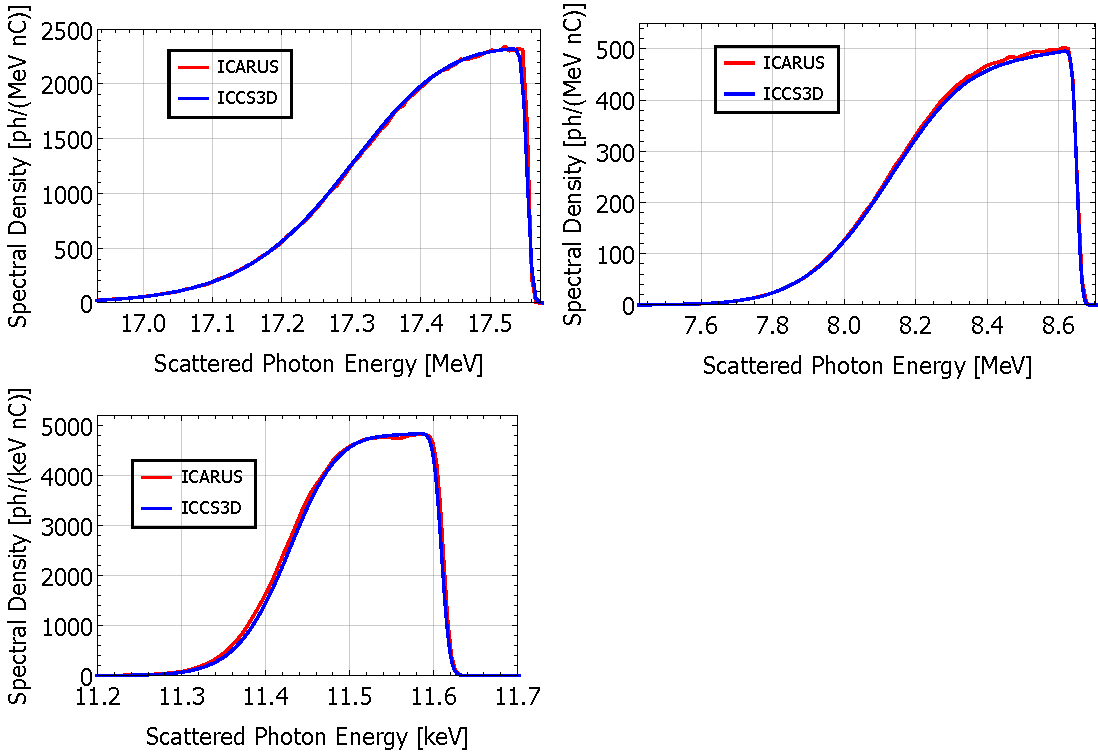
\includegraphics[width=\textwidth]{Figures/Optimisation_and_Characterisation_of_Inverse_Compton_Scattering_Sources/ICARUS_ICCS3D_cases_comparison.pdf}
\caption{Comparison of ICS head-on ($\phi=0$) single electron bunch--laser pulse interaction spectra using circular collimation for each case in Table~\ref{tab:char_opt_electron_bunch_parameters}, produced by the semi-analytical codes \textsc{ICARUS} (red) and \textsc{ICCS3D} (blue) for 0.5\% \textit{rms} (2\% case B) bandwidth, with configuration optimised by the single point GA non-round beam optimisation  (see Section~\ref{sec:NRB_optimisation}). All \textsc{ICARUS} spectra are produced using $100\times 10^{6}$ QMC points and sampled at 100 points across the energy range. Top Left: Case A. Top Right: Case B. Bottom Left: Case C.}
\label{fig:ICARUS_optimised_benchmarking}
\end{figure}

The \textsc{ICARUS} and \textsc{ICCS3D} spectra for cases A, B and C in Fig.~\ref{fig:ICARUS_optimised_benchmarking} show good agreement. The spectra in each case produced via \textsc{ICARUS} and \textsc{ICCS3D} are near-identical in shape, with identical peak spectral density and Compton edge energies (Eq.~\ref{eq:compton_edge_energy}) -- the scattered photon energy at peak spectral density -- in both of the spectra for each case. Consequently, the spectral yield (collimated flux) is in good agreement between the two codes -- an agreement in collimated flux of $< 2\%$ is noted for each of the benchmarking cases.

% Explain features of spectra
The spectra have a high energy tail resulting from the energy spread of the electron bunch and laser pulse spectral bandwidth at low spectral densities. Peak spectral density is the location of the Compton edge, with scattered photon energy given by (Eq.~\ref{eq:compton_edge_energy}), which corresponds to the centroid energy of the electron bunch and laser pulse and occurs in the back-scattered direction ($\theta=0$). The collimator truncates the spectrum, so we do not see the full ICS source spectrum as shown in Fig.~\ref{fig:cross_section_scattered_photon_energy}. Emittance of the electron bunch and collimation result in the shape of the low energy tail of the spectrum. 

Through collaboration with the \textsc{ICCS3D} \cite{krafft2016laser,ranjan2018simulation,terzic2019improving} designers and benchmarking with \textsc{ICARUS} an integration problem has been noted in \textsc{ICCS3D} where the spectrum code was producing incorrect results for long electron bunch and laser pulse lengths, which was corrected during benchmarking for the CBETA ICS source in Chapter~\ref{CBETA_Inverse_Compton_Scattering_Source_Design}.
\textsc{ICCS3D} was previously quoted in arbitrary units because it was benchmarked against the spectrum model by Sun et al \cite{sun2009characterizations}, which contained the inverse square law error described in Section~\ref{sec:development_of_the_ICARUS_spectrum_code}. Through understanding of the inverse square law error and the good agreement shown in Fig.~\ref{fig:ICARUS_optimised_benchmarking} the arbitrary units could be replaced with the proper units of the spectral density, allowing \textsc{ICARUS} and \textsc{ICCS3D} to quantitatively predict the results of ICS experiments.   

However, oscillatory behaviour or `roughness' -- quickly varying amplitude of the spectral density -- is present in the shape of the \textsc{ICARUS} spectra because of the highly oscillatory integrals involved in the electron bunch energy spread term of (Eq.~\ref{eq:ICARUS_equation}) with small electron bunch energy spread
\begin{equation}
\frac{dN_{\gamma}}{dE_{\gamma}} &\propto \exp\left[\frac{\left(\gamma-\gamma_{0}\right)^{2}}{2\sigma_{\gamma}^{2}}\right],
\label{eq:ICARUS_electron_energy_spread_term}
\end{equation}
which causes errors in the quasi-Monte Carlo integration. The 'roughness` effect appears unphysical and, upon further investigation, seems related to the number of quasi-Monte Carlo integration points used in the simulation. 

Therefore, two simulation parameters which could affect the quality of the \textsc{ICARUS} simulation have been further investigated: the number of simulation points calculated for the model (Eq.~\ref{eq:ICARUS_equation}) and the number of quasi-Monte Carlo points used in the integration. Both have been investigated using case A in Table~\ref{tab:char_opt_electron_bunch_parameters}, with collimation and $\beta$-functions at the IP specified by a 0.5\% \textit{rms} bandwidth optimisation using the non-round beam genetic algorithm method ($\theta_{\mathrm{col}}=0.066$~\si{\milli\radian}, $\beta_{x}^{*}=2.11$~\si{\meter}, $\beta_{y}^{*}=0.867$~\si{\meter}), as is used in Fig.~\ref{fig:ICARUS_optimised_benchmarking}. The investigation into the study of the number of simulation points produces \textsc{ICARUS} spectra with a range of 10--300 simulation points and a constant $5\times 10^{7}$ QMC points. Whereas the study of the number of QMC points produces \textsc{ICARUS} spectra with 100 simulation points and 10--100 million QMC points. The results of the simulation and QMC point investigations are shown in Fig.~\ref{fig:ICARUS_sim_qmc_points}

\begin{figure}[!h]
\centering
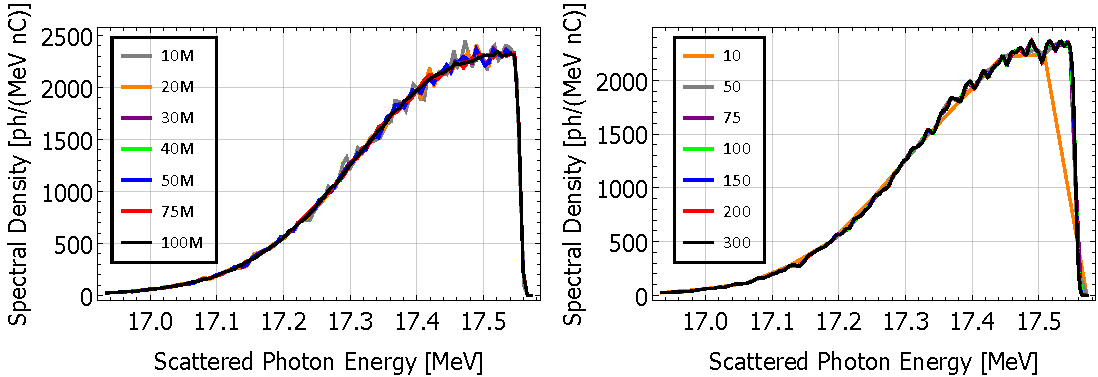
\includegraphics[width=\textwidth]{Figures/Optimisation_and_Characterisation_of_Inverse_Compton_Scattering_Sources/QMC_SIM_POINT_STUDY.pdf}
\caption{Left: A series of \textsc{ICARUS} spectra for varying number of quasi-MonteCarlo points (M=million) used within the integration routine, performed for 100 simulation points using Case A. More integration points produce a smoother spectrum -- the oscillations in the spectra are due to integration errors. Right: A series of \textsc{ICARUS} spectra for varying number of simulation points, performed with 50 million QMC points using Case A. Too few points results in a poorly defined spectra.}
\label{fig:ICARUS_sim_qmc_points}
\end{figure}

% write about all that
The study of the number of simulations points shows that the spectrum is poorly defined and hard-edged for a low number of simulation points, for example the 10 simulation points spectrum in Fig.~\ref{fig:ICARUS_sim_qmc_points}. Beyond $\sim100$ simulation points the shape of the spectrum is not noticeably improved, therefore 100 simulation points is a reasonable number of simulation points for an \textsc{ICARUS} simulation. The simulation time increases near-linearly with increasing simulation points; with 100 simulation points the simulation time is 64~\si{\minute} and 300 simulation points requires 194~\si{\minute}. Therefore $>100$ simulation points only increases the time of the simulation not the quality.

In Fig.~\ref{fig:ICARUS_sim_qmc_points}, the \textsc{ICARUS} spectra are shown for varying quantities of quasi-Monte Carlo integration points; the spectral shape improves with number of quasi-Monte Carlo points utilised as the `roughness' of the spectral shape is removed. The `roughness' is deemed unphysical because the amplitude of the spectral density oscillations present in the case A spectrum are reduced with additional quasi-Monte Carlo integration points which increase the accuracy of the integration. However, increasing the number of QMC points used in the simulation increases the simulation time. For example, a 100 million QMC point \textsc{ICARUS} simulation increases the simulation time $\sim 12$ fold over a 10 million QMC point simulation.    

\subsection{Analytical Collimated Flux}
\label{sec:analytical_collimated_flux_benchmarking}

The analytical collimated flux (Eq.~\ref{eq:collimated_flux}) derived in Section~\ref{sec:analytical_collimated_flux} has been compared against numerous methods including the analytical formulation by Curatolo et al \cite{curatolo2017analytical} as well as the collimated flux (spectral yield) calculated from the \textsc{ICARUS} and \textsc{ICCS3D} \cite{krafft2016laser,ranjan2018simulation} spectrum codes. The collimated flux is calculated by Curatolo et al, in `natural units' as 
\begin{equation}
\mathcal{F}_{\mathrm{col}} = 6.25\times 10^{8}\frac{E_{\mathrm{pulse}}\left(\mathrm{\si{\joule}}\right)Q\left(\si{\pico\coulomb}\right)f\left(\si{\hertz}\right)}{E_{L}\left(\si{\electronvolt}\right)\left[\sigma_{e}^{2}\left(\si{\micro\meter}\right)+\sigma_{L}^{2}\left(\si{\micro\meter}\right)\right]}\times\frac{\left(1+\sqrt[3]{X}\Psi^{2}/3\right)\Psi^{2}}{\left[1+\left(1+X/2\right)\Psi^{2}\right]\left(1+\Psi^{2}\right)},
\label{eq:curatolo_collimated_flux}
\end{equation}
where all aymbols are consistent with those in (Eq.~\ref{eq:collimated_flux}), $\Psi-\gamma\theta_{\mathrm{col}}$ is the acceptance angle and $\sigma_{e} = \sqrt{\sigma_{x}^{2}+\sigma_{y}^{2}}$ is the \texit{rms} spot size of the electron bunch at the IP, with $\sigma_{x/y}$ the \textit{rms} spot size in each plane.

The collimated flux calculation by Curatolo et al \cite{curatolo2017analytical} (Eq.~\ref{eq:curatolo_collimated_flux}) uses the Berestetskii, Pitaevskii and Lifshitz \cite{berestetskii1982quantum} differential cross section (Eq.~\ref{eq:differential_cross_section_Y_invariant}) like the derivation presented here in Section~\ref{sec:analytical_collimated_flux} however, an explicit derivation is not shown or referenced. Upon inspection of (Eq.~\ref{eq:curatolo_collimated_flux}), it is evident that this is only valid for a head-on ($\phi=0$) interaction and doesn't account for the  hourglass effect \cite{furman1991hourglass,miyahara2008luminosity} -- the luminosity reduction due to interaction of a diverging laser pulse and electron bunch -- outlined in Section~\ref{sec:geometric_luminosity_reduction}. Therefore, to align the Curatolo et al calculations (Eq.~\ref{eq:curatolo_collimated_flux}) with (Eq.~\ref{eq:collimated_flux}), the angular crossing and hourglass effect luminosity reduction factor $R_{ACHG}$ \cite{miyahara2008luminosity} (Eq.~\ref{eq:miyahara_combined_reduction}) must be introduced.

The collimated flux calculation methods are compared using the benchmarking cases in Section~\ref{sec:benchmarking_cases_characterisation_optimisation} with the electron bunch parameters in Table~\ref{tab:char_opt_electron_bunch_parameters} and laser pulse parameters in Table~\ref{tab:char_opt_laser_pulse_parameters}. The calculations have been conducted using the genetic algorithm single point bandwidth optimisation, as outlined in Section~\ref{sec:NRB_optimisation}, for a 0.5\% \textit{rms} bandwidth (2\% \textit{rms} bandwidth case B) which yields the values for the $\beta$-functions at the IP and collimation angle shown later in this chapter in Table~\ref{tab:single_point_optimisations}. The results of the collimated flux calculations, by each method, for each of the benchmarking cases A, B and C are shown in Table~\ref{tab:collimated_flux_calculations}

\begin{table}[!h]
\centering
\caption{Calculations of collimated flux in a 0.5\% \textit{rms} bandwidth (Case B 2\% \textit{rms} bandwidth) for each of the benchmarking cases in Table~\ref{tab:char_opt_electron_bunch_parameters}, using non-round beam genetic algorithm interaction point parameters as shown in Table~\ref{tab:single_point_optimisations}, via a variety of methods. Laser parameters shown in Table~\ref{tab:char_opt_laser_pulse_parameters} are kept constant for each benchmarking case.}
\vspace{3mm}
\begin{threeparttable}
\begin{tabular}{lccc}
\hline\hline
 & \multicolumn{3}{c}{Collimated Flux (ph/\si{\second})} \\
\hline
Method & Case A & Case B & Case C \\
\hline 
Curatolo et al~\tnote{*} (Eq.~\ref{eq:curatolo_collimated_flux}) \cite{curatolo2017analytical} & $6.03 \times 10^{8}$ & $5.95\times 10^{9}$ & $7.35\times 10^{7}$ \\
Analytical (Eq.~\ref{eq:collimated_flux}) & $8.86 \times 10^{8}$ & $1.04 \times 10^{10}$ & $1.17\times 10^{8}$ \\
\textsc{ICARUS}~\tnote{$\dagger$} (Eq.~\ref{eq:spectral_yield}) & $8.76\times 10^{8}$ & $1.04\times 10^{10}$ & $1.14\times 10^{8}$ \\
\textsc{ICCS3D}~\tnote{$\dagger$} (Eq.~\ref{eq:spectral_yield}) \cite{krafft2016laser,ranjan2018simulation} & $8.75\times 10^{8}$ & $1.02\times 10^{10}$ & $1.16\times 10^{8}$  \\
\hline\hline
\end{tabular}
\begin{tablenotes}
\item[*]{The Curatolo et al collimated flux (Eq.~\ref{eq:curatolo_collimated_flux}) has been multiplied by the combined angular crossing and hourglass effect luminosity reduction factor (Eq.~\ref{eq:miyahara_combined_reduction}) for comparison with other collimated flux calculations.}
\item[$\dagger$]{The \textsc{ICARUS} and \textsc{ICCS3D} spectra used in the calculation of the collimated flux (spectral yield) are shown in Fig.~\ref{fig:ICARUS_optimised_benchmarking}.}
\end{tablenotes}
\end{threeparttable}
\label{tab:collimated_flux_calculations}
\end{table}

The collimated flux calculations in Table~\ref{tab:collimated_flux_calculations} show good agreement between the spectrum code calculations, as \textsc{ICARUS} and \textsc{ICCS3D} agree to within $< 2\%$ in all cases. Good agreement was shown qualitatively between these two codes in Fig.~\ref{fig:ICARUS_optimised_benchmarking}, therefore good quantitative agreement was expected. Between the \textsc{ICARUS} code and the analytical collimated flux calculation (Eq.~\ref{eq:collimated_flux}), a maximum discrepancy of 1.14\% is observed. Percentage scale discrepancies between these two calculations can be expected because the analytical calculation neglects the energy spread of the electron bunch and the spectral bandwidth of the laser pulse and the \textsc{ICARUS} code is not exact because of oscillatory integration errors, as discussed in Section~\ref{sec:ICARUS_benchmarking}. 

However, the collimated flux calculation by Curatolo et al \cite{curatolo2017analytical} (Eq.~\ref{eq:curatolo_collimated_flux}) shows large discrepancies from both the analytical collimated flux derived in Section~\ref{sec:analytical_collimated_flux} and the spectrum codes. Table~\ref{tab:collimated_flux_calculations} shows the Curatolo et al collimated flux (Eq.~\ref{eq:curatolo_collimated_flux}) is consistently reduced with reference to the analytical (Eq.~\ref{eq:collimated_flux}) and spectrum code collimated flux, which is also observed in Fig.~\ref{fig:curatolo_collimated_flux_comparison}. For example, in Table~\ref{tab:collimated_flux_calculations}, a factor $\sim 1.75$ reduction in collimated flux is observed between (Eq.~\ref{eq:collimated_flux}) and (Eq.~\ref{eq:curatolo_collimated_flux}) for case B. The discrepancy must originate in the angular term of (Eq.~\ref{eq:curatolo_collimated_flux})
\begin{equation*}
\mathcal{F}_{\mathrm{col}}\propto\frac{\left(1+\sqrt[3]{X}\Psi^{2}/3\right)\Psi^{2}}{\left[1+\left(1+X/2\right)\Psi^{2}\right]\left(1+\Psi^{2}\right)}    
\end{equation*}
because the head-on luminosity is equivalent in both equations, the geometric luminosity reduction is applied identically and the cross section variation of Case A (the maximum electron bunch energy case, $E_{e}=1$~\si{\giga\electronvolt}) is small -- a 1.2\% reduction in the ICS cross section (Eq.~\ref{eq:compton_cross_section_classical_limit}). The cross section variation with electron energy is illustrated in Fig.~\ref{fig:cross_section_electron_energy}. However, the origin of the discrepancy in the angular term of the Curatolo et al \cite{curatolo2017analytical} calculation (Eq.~\ref{eq:curatolo_collimated_flux}) remains unknown because no adequate derivation is shown within the literature.   

To further investigate the angular dependency of the collimated flux calculations the collimated flux, via the two analytical methods (Eqs.~\ref{eq:collimated_flux}, \ref{eq:curatolo_collimated_flux}) and the \textsc{ICARUS} spectrum code, has been calculated as a function of the acceptance angle in Fig.~\ref{fig:curatolo_collimated_flux_comparison}. The benchmarking cases from Table~\ref{tab:char_opt_electron_bunch_parameters} are used, where the interaction $\beta$-functions are those from the 0.5\% \textit{rms} bandwidth (case B 2\% \textit{rms} bandwidth) non-round beam genetic algorithm optimisation, and the collimation angle is varied. Laser parameters remain constant, as given in Table~\ref{tab:char_opt_laser_pulse_parameters}. 
  
\begin{figure}[!h]
\centering
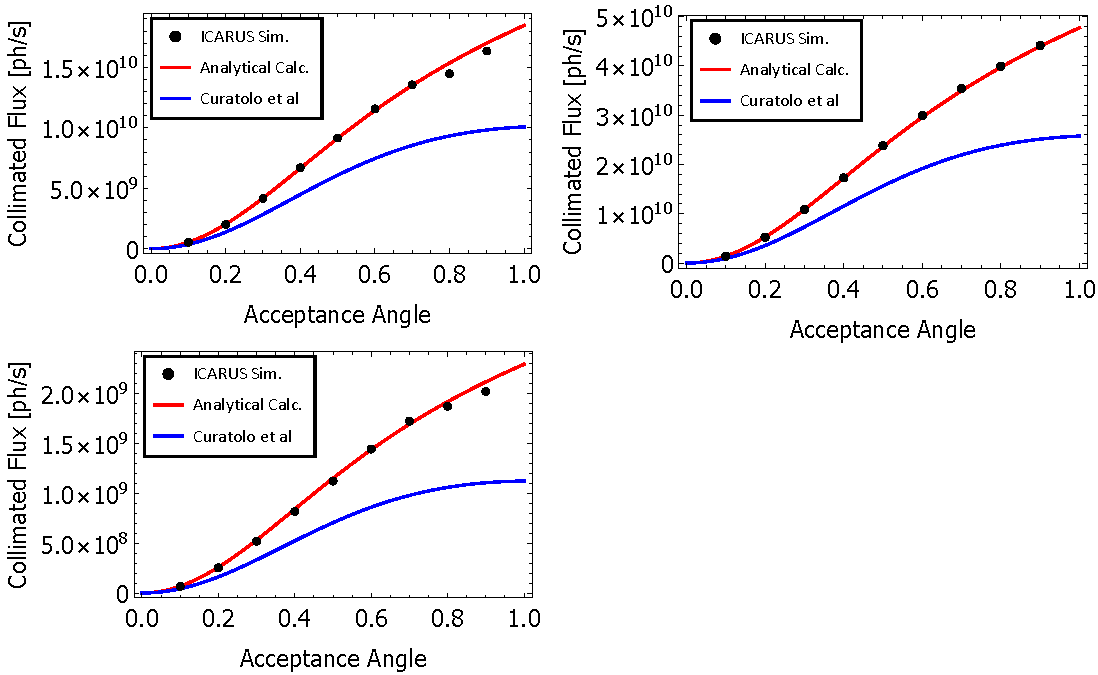
\includegraphics[width=\textwidth]{Figures/Optimisation_and_Characterisation_of_Inverse_Compton_Scattering_Sources/Fcol_PSI_Cases_Curatolo_Analytical_ICARUS.pdf}
\caption{Comparison of the derived analytical collimated flux (Eq.~\ref{eq:collimated_flux}) (blue) with the Curatolo et al collimated flux calculation \cite{curatolo2017analytical}  (Eq.~\ref{eq:curatolo_collimated_flux}) (red) and the results of the \textsc{ICARUS} spectrum code (black) (50 million QMC, 100 sim points) within an acceptance angle $0 \geq \Psi \geq 1$ (a $1/\gamma$ cone). The benchmarking cases presented in Table~\ref{tab:char_opt_electron_bunch_parameters}, optimised for a 0.5\% \textit{rms} bandwidth (Case B 2\% \textit{rms} bandwidth) using the non-round beam genetic algorithm with parameters shown in Table~\ref{tab:single_point_optimisations}. The \textsc{ICARUS} spectrum code data has been adjusted for an angular crossing (Eq.~\ref{eq:angular_crossing_factor}) and the Curatolo et al calculation (Eq.~\ref{eq:curatolo_collimated_flux}) has been adjusted for the hourglass effect and angular crossing (Eq.~\ref{eq:miyahara_combined_reduction}). Top Left: Case A. Top Right: Case B. Bottom Left: Case C.}
\label{fig:curatolo_collimated_flux_comparison}
\end{figure}

In Fig.~\ref{fig:curatolo_collimated_flux_comparison}, there is a strong agreement between the analytical collimated flux and that derived from the \textsc{ICARUS} spectrum code, therefore (Eq.~\ref{eq:scattered_photon_energy}) can efficiently predict the collimated flux across the whole range of scattering angles. However, at large acceptance angles in case A and C the \textsc{ICARUS} values differ from the analytical calculation. The discrepancy is due to using 50 million QMC points, which can result in a small integration error, as previously shown in Fig.~\ref{fig:ICARUS_sim_qmc_points}, and also from using only 100 simulation points in each simulation. The scattered photon energy range increases with collimation angle because of the energy--angle correspondence  in the scattered photon energy (Eq.~\ref{eq:scattered_photon_energy}) which, with a constant 100 simulation points, dilutes the spectrum as the step energy between simulation points is greater. The collimated flux calculation by Curatolo et al \cite{curatolo2017analytical} (Eq.~\ref{eq:curatolo_collimated_flux}) disagrees with (Eq.~\ref{eq:collimated_flux}) and the \textsc{ICARUS} scattering code beyond $\psi>0.1$ in each case in Fig.~\ref{fig:curatolo_collimated_flux_comparison}. The discrepancy in the Curatolo et al calculation increases as a function of acceptance angle, which suggests that a small angle approximation could occur within the derivation of (Eq.~\ref{eq:curatolo_collimated_flux}), however it is unverifiable because (Eq.~\ref{eq:curatolo_collimated_flux}) is not derived in the literature.  

The analytical calculation (Eq.~\ref{eq:collimated_flux}) is proficient at calculating the yield of ICS spectrum codes within energy spread and spectral bandwidth tolerances and consequently is a valid alternative to spectrum code collimated flux calculations. The analytical collimated flux calculation is advantageous in terms of simulation time, as the collimated flux is calculated analytically on a sub-second timescale whereas the spectrum codes at 100 million QMC points and 100 simulation points require hours to run. Consequently, the analytical collimated flux is a useful calculation method for computing the many collimated flux values required in the optimisations detailed in the rest of this chapter.   

\section{Motivation for Narrowband Optimisation of ICS Sources}
\label{sec:motivation_optimisation}

Currently, many ICS sources \cite{deitrick2017inverse,deitrick2018high,pan2019design,dupraz2020thomx} are designed to produce maximise uncollimated flux. However, ICS sources used for light source experimentation have two objectives: to produce a large quantity of photons and to minimise the energy spread (bandwidth) of the scattered radiation towards a monochromatic source, using a collimator. The former, a high flux of photons, is desirable because a high flux increases data acquisition times and improves the signal-to-noise ratio of measurements and the latter is advantageous due to the ability to target certain process with small energy acceptances, for example a specific resonance in an isotope like $^{235}\mathrm{U}$ for a nuclear resonance fluorescence investigation \cite{hayakawa2010nondestructive}. Users typically require a compromise on bandwidth and flux for precise investigations of specific energy dependent phenomena whilst conducting measurements on a reasonable timescale, with adequate statistics. Therefore, within the following optimisations we aim to maximise the collimated flux (Eq.~\ref{eq:collimated_flux}) whilst minimising, or limiting to some user specified value, the \textit{rms} bandwidth (Eq.~\ref{eq:RMS_bandwidth}) of the ICS source. All optimisations are performed with the assumption of a circular collimator, as the focus of this study is on narrow bandwidth and studies by Hajima \cite{hajima2021bandwidth} demonstrate circular collimation is the optimum approach for narrow bandwidth; the analytical collimated flux (Eq.~\ref{eq:collimated_flux}) is also derived for circular collimation.

To maximise the collimated flux within a user determined bandwidth the transverse dynamics of the electron bunch and the collimation are modified. Variables include the $\beta$-functions of the electron bunch at the IP $\beta^{*}_{x/y}$ and the collimation angle $\theta_{\mathrm{col}}$; justification for these choices is provided in Section~\ref{sec:objective_functions_and_variables}. Therefore, maximising collimated flux for a specific bandwidth is a multi-dimensional multi-objective optimisation problem with up to 3 variables and 2 objective functions. Local optimisation techniques may be insufficient because the parameter space of this optimisation is non-linear -- the objective functions do not vary linearly with the variables -- and the complexity of the parameter space is unknown; consequently both global and local optimisation techniques are trialed.

Transverse electron bunch dynamics are selected for optimisation as preliminary scaling studies showed adjustment of electron bunch interaction parameters to be a viable method of increasing the collimated flux and bandwidth. In comparison, optimising the transverse IP dynamics of the laser pulse is more complex because Fabry-Perot optical cavity design is severely constrained, as discussed in Section~\ref{sec:lasers_fabry_perot}. Electron bunch longitudinal dynamics could also be considered for optimisation of the collimated flux and bandwidth because the bandwidth (Eq.~\ref{eq:RMS_bandwidth}) is dependent on the electron bunch energy spread and the collimated flux is (weakly) dependent on the electron bunch length. Transverse electron bunch optimisation is favoured to longitudinal optimisation because the collimated flux advantage is small, due to the weak electron bunch length dependence, longitudinal optimisation is also more complex because of the RF system -- requiring a more complete accelerator design. Transverse laser pulse and longitudinal electron bunch optimisations are suitable subjects for future work.  

In the second half of this chapter the objective functions and variables of the optimisations are justified and a default ICS source configuration -- transverse profile matching (TPM) -- applied to maximise the flux of many ICS sources is explained. Several optimisation methods are then developed in this chapter: a round beam optimisation (RB) (Section~\ref{sec:RB_optimisation}), a non-round beam simplex optimisation (NRB simplex) and a non-round beam genetic algorithm method (NRB GA) are developed and tested in Section~\ref{sec:NRB_optimisation} to optimise the multi-objective collimated flux--\textit{rms} bandwidth problem. Each optimisation method is first demonstrated using benchmarking case A in Table~\ref{tab:char_opt_electron_bunch_parameters}, with laser parameters in Table~\ref{tab:char_opt_laser_pulse_parameters}, before all benchmarking cases are used to evaluate the optimisation methods in Section~\ref{sec:evaluation_of_optimisation_methods}.

Round beam optimisations simplify the transverse dynamics so they are identical in each plane ($x$ and $y$), whereas non-round beam optimisations treat each transverse plane individually. The round beam optimisation in Section~\ref{sec:RB_optimisation} uses a brute force optimisation approach, calculating each possible solution then sorting for the best solution. More sophisticated algorithms are required for non-round beams because the parameter space is significantly expanded and unbounded. Developed non-round beam optimisations use a downhill simplex method, based on the Nelder-Mead NMaximise routine in \textsc{Mathematica} \cite{wolfram2021nmaximize}, and the upgraded strength Pareto evolutionary algorithm (\textsc{SPEA2}) \cite{zitzler2001spea2} -- a genetic algorithm (GA) -- with the \textsc{PISA} platform \cite{bleuler2003pisa}, where a series of \textsc{Python} scripts have been wrote to interface with the generalised multi-objective evolutionary optimisation code. These optimisation methods are applied, in various forms, throughout the ICS source designs in Chapters~\ref{CBETA_Inverse_Compton_Scattering_Source_Design} and \ref{DIANA_Inverse_Compton_Source_Design}.    

\section{Objective Functions and Variables}
\label{sec:objective_functions_and_variables}

Two competing objective functions are used to optimise an ICS source: the collimated flux (Eq.~\ref{eq:collimated_flux}), which is maximised, and \textit{rms} bandwidth (Eq.~\ref{eq:RMS_bandwidth}), which is minimised. Extension to the FWHM bandwidth (Eq.~\ref{eq:FWHM_bandwidth}) is trivial. The analytical calculation of the collimated flux (Eq.~\ref{eq:collimated_flux}) is favoured over the \textsc{ICARUS} code because, whilst the \textsc{ICARUS} code is more accurate, using \textsc{ICARUS} is time prohibitive, as discussed in Section~\ref{sec:analytical_collimated_flux_benchmarking}. The two objective functions compete; minimising the two dominant terms of the \texit{rms} bandwidth (Eq.~\ref{eq:RMS_bandwidth}), the emittance/divergence term (Eq.~\ref{eq:emittance_term}) and the collimation term (Eq.~\ref{eq:collimation_term}), reduces the collimated flux. Therefore, a trade-off between the competing objectives is developed -- maximisation of the collimated flux within a user selected \textit{rms} bandwidth. 

Optimisation of the ICS interaction aims to both produce the optimum configuration for a particular ICS source experiment and also allow the parameter space of the ICS source to be mapped. Tuning curves, where a Pareto front is generated in collimated flux--\textit{rms} bandwidth space, map the possible configurations of an ICS source. Whereas a single bandwidth point optimisation, where the $\textit{rms}$ bandwidth objective is replaced by a penalty function 
\begin{equation}
\Omega = \left|\left(\frac{\Delta E_{\gamma}}{E_{\gamma}}\right)_{\mathrm{tar}}-\left(\frac{\Delta E_{\gamma}}{E_{\gamma}}\right)_{\mathrm{ach}}\right|,
\label{eq:penalty_function}
\end{equation}
where $\left(\Delta E_{\gamma}/E_{\gamma}\right)_{\mathrm{tar}}$ is the user targeted bandwidth and $\left(\Delta E_{\gamma}/E_{\gamma}\right)_{\mathrm{ach}}$ is the bandwidth achieved by the optimisation, determines the optimal electron bunch and collimation settings for a particular experiment. Here, methods are developed to perform both tuning curve optimisations and single point optimisations.

Inspection of the \textit{rms} bandwidth for ICS sources has shown that the emittance (Eq.~\ref{eq:emittance_term}) and collimation (Eq.~\ref{eq:collimation_term}) terms are frequently the dominant terms, which are dependent upon the transverse $\beta$-functions at the IP $\beta^{*}_{x/y}$ in each plane, the emittance (emittance term) in each plane and the collimation angle $\theta_{\mathrm{col}}$ (collimation term) respectively. Similarly, the collimated flux (Eq.~\ref{eq:collimated_flux}) shares a dependency upon these parameters so these are adequate candidates for optimisation. Varying the $\beta$-functions at the IP is favoured because the $\beta$-functions can be varied through adjustment of the final focus system whereas the transverse emittance is dependent on the electron photo-injector and the collective effects experienced by the bunch throughout the accelerator, from generation of the bunch to interaction. Collimation of the produced radiation is external to the electron bunch--laser pulse interaction, therefore collimation angle is an easy parameter to adjust by using a selection of collimators, a variable aperture collimator or by adjusting the source-to-collimator distance. The chosen ICS source IP variables ($\beta^{*}_{x}$, $\beta^{*}_{y}$, $\theta_{\mathrm{col}}$) can be tuned for any accelerator type generalising the optimisation to any accelerator driver of an ICS source, not just an ERL.

Limitations of final focuses imposed in ICS sources mean the $\beta$-functions at the IP are realistically lower bounded to the \si{\milli\meter}-scale ($\beta_{x/y}^{*} > 1$~\si{\milli\meter}), such as the 0.48~\si{\milli\meter} $\beta$-function at the KEK ATF2 \cite{okugi2016achievemen} used as a demonstrator for the international linear collider (ILC) \cite{yamamoto2021international}. The upper bound of the $\beta^{*}$-functions is optimisation case specific; an upper limit can be derived in the round beam case (see Section~\ref{sec:RB_optimisation}) but upper bounds must be arbitrarily specified in the non-round beam case in Section~\ref{sec:NRB_optimisation}, since the $\beta$-functions are unbounded. The collimation angle is lower bounded as the collimation angle must be larger than zero ($\theta_{\mathrm{col}}>0$) -- or the collimator becomes an attenuator -- and is upper bounded through the assumption that the collimation term (Eq.~\ref{eq:collimation_term}) is dominant and the \textit{rms} bandwidth (Eq.~\ref{eq:RMS_bandwidth}) becomes
\begin{equation}
\left(\frac{\Delta E_{\gamma}}{E_{\gamma}}\right)_{\mathrm{rms}} \approx \left(\frac{\sigma_{\theta}}{E_{\theta}}\right),    
\label{eq:collimation_dominant}
\end{equation}
which, by expanding the collimation term (Eq.~\ref{eq:collimation_term}), is re-cast as an approximate collimation angle upper bound  
\begin{equation}
\theta_{\mathrm{col},\mathrm{max}} \approx \frac{1}{\gamma}\sqrt{\frac{2\sqrt{3}\left(\Delta E_{\gamma}/E_{\gamma}\right)_{\mathrm{rms}}\left[1+X\right]}{1-\sqrt{3}\left(\Delta E_{\gamma}/E_{\gamma}\right)_{\mathrm{rms}}}}
\label{eq:collimation_angle_upper_bound}    
\end{equation}
where all terms have previously been defined and $0<\theta_{\mathrm{col}}<\theta_{\mathrm{col},\mathrm{max}}$.

\section{Transverse Profile Matching}
\label{sec:transverse_profile_matching}

Many inverse Compton scattering sources have attempted to maximise uncollimated flux output via matching the transverse \textit{rms} spot size of the laser pulse to that of the electron bunch ($\sigma_{L}\approx\sigma_{\mathrm{electron}}$) \cite{akagi2016narrow,deitrick2018high,jacquet2015radiation,drebot2019brixs}, termed here the transverse profile matching (TPM) scheme. The transverse profile matching scheme ignores the full interaction dynamics at the IP in favour of a simplistic solution, which is a sensible first order approximation. 

Matching the spot sizes of the electron bunch and laser pulse means the collimation angle is the only free parameter to control the bandwidth of the ICS source. However, the emittance term of the bandwidth (Eq.~\ref{eq:emittance_term}) is the dominant bandwidth term, unless emittance is small ($\epsilon_{n} < 1$~\si{\milli\meter}-\si{\milli\radian}). For example, using case B in Table~\ref{tab:char_opt_electron_bunch_parameters}, the emittance term for transverse profile matching exceeds the collimation term (Eq.~\ref{eq:collimation_term}) up until $\theta_{\mathrm{col}} = 4.25$~\si{\milli\radian}. Therefore, with a collimation angle as a singular variable achieving narrow bandwidth without small emittance is not possible. Transverse profile matching also doesn't account for scenarios such as case A (Table~\ref{tab:char_opt_electron_bunch_parameters}), with small emittance, where the laser pulse spot size at the IP is large and higher flux is possible via reduced electron bunch spot size at the IP. 

The intensity of the laser pulse and electron bunch are often non-uniform transversely (for example in a Gaussian laser pulse), and instead intensity peaks at the centroid. A laser pulse used in inverse Compton scattering is typically orders of magnitude more intense than the electron bunch ($N_{L} \gg N_{e}$), for example a 1~\si{\nano\coulomb} bunch contains $N_{e} = 6.25\times 10^{9}$ electrons and a paltry 1~\si{\micro\joule} Nd:YAG ($\lambda = 1064$~\si{\nano\meter}) laser pulse contains $N_{L} = 5.35\times 10^{12}$ photons. Therefore, to maximise the probability of electron--photon interaction it is favourable to obey the condition $\sigma_{L} > \sigma_{\mathrm{electron}}$.

To first order, the transverse profile matching scheme is a decent approximation for interaction between laser pulse profiles chosen to avoid the worst diffraction effects and near-round transverse electron bunches  ($\sigma_{x,\mathrm{electron}}\sim\sigma_{y,\mathrm{electron}}$) delivered by an ERL or linac. Within experimental tolerances, such as electron beam jitter, alignment of the laser and electron beam transverse profile matching may be the most attractive scenario, and further work is required to understand experimental tolerances. However for an ICS light source, high flux narrow-bandwidth operation is necessary and optimisation of transverse interaction point parameters offers improvement over TPM schemes. 

\section{Round Beam Optimisation}
\label{sec:RB_optimisation}

Here we develop a brute-force global optimisation method to maximise flux within a selected \textit{rms} bandwidth for the simplified case of an electron beam with a round transverse profile where the normalised emittance and $\beta$-functions at the IP are assumed to be identical in both planes ($\epsilon_{nx} = \epsilon_{ny} = \epsilon_{n}$, $\beta_{x}^{*} = \beta_{y}^{*} = \beta^{*}$), named the round beam (RB) approximation. Consequently, bandwidth tuning is possible via two variables: selecting $\beta^{*}$ at the IP and by setting the collimation angle $\theta_{\mathrm{col}}$. The $\beta$-function at the IP is selected over the emittance, as discussed in Section~\ref{sec:objective_functions_and_variables}. The round beam approximation simplifies the interaction dynamics from the full non-round beam model, with three variables. RB optimisation shows simple optimisation can yield improvement in collimated flux, and is applicable in ICS sources with near-round electron bunch transverse profiles -- as in ERLS and linacs.

For the RB optimisation, the \textit{rms} bandwidth is given by (Eq.~\ref{eq:RMS_bandwidth}) with the emittance term (Eq.~\ref{eq:emittance_term}) modified for the transversely round bunch case
\begin{equation}
\frac{\sigma_{\epsilon}}{E_{\epsilon}} = \frac{2\gamma\epsilon_{n}}{\left(1+X\right)\beta^{*}},
\label{eq:emittance_term_round_beam}    
\end{equation}
where $X$ is the recoil parameter (Eq.~\ref{eq:X_geometry}), $\epsilon_{n}$ is the transverse \textit{rms} normalised emittance of the electron bunch and $\beta^{*}$ is the $\beta$-function at the interaction point. As mentioned in Section~\ref{sec:objective_functions_and_variables}, the collimation term Eq.~(\ref{eq:collimation_term}) and the emittance term Eq.~(\ref{eq:emittance_term_round_beam}) are dominant. Therefore, optimisation of bandwidth and collimated flux minimises the collimation and emittance terms whilst maximising collimated flux.

By using a larger $\beta^{*}$ and a small collimator aperture (collimation angle), the contribution of the collimation and emittance terms can be reduced so that they are negligible; thus the electron bunch (Eq.~\ref{eq:beam_energy_spread_term}) and laser pulse energy spread terms (Eq.~\ref{eq:laser_energy_spread_term}) dominate the bandwidth for accelerators with a sufficiently small emittance. Taking the limit of a small collimation angle ($\theta_{\mathrm{col}}\rightarrow 0$), and assuming the $\beta$-function at the IP can be made very large ($\beta^{*}\rightarrow 0$) this effectively places a lower limit on the bandwidth of an ICS source; it is limited by the energy spread of the electron beam $\Delta E_{e}/E_{e}$ and laser pulse spectral bandwidth $\Delta E_{\mathrm{laser}}/E_{\mathrm{laser}}$ as 
\begin{equation}
\left(\frac{\Delta E_{\gamma}}{E_{\gamma}}\right)_{\mathrm{min}} \approx \sqrt{\left[\left(\frac{2+X}{1+X}\right)\frac{\Delta E_{e}}{E_{e}}\right]^{2} + \left[\left(\frac{1}{1+X}\right)\frac{\Delta E_{L}}{E_{L}}\right]^{2}}.
\label{eq:bandwidth_limitation_minimum}
\end{equation}

Consequently, any bandwidth above the 
limit (Eq.~\ref{eq:bandwidth_limitation_minimum}) can theoretically be achieved by an ICS source by tuning of the collimation angle and $\beta$-function at the IP so that a desired bandwidth, $\Delta E_{\gamma}/E_{\gamma}$, is achieved. Since the collimation and emittance terms are typically dominant, all other terms can be excluded and the solutions are approximately bounded by
\begin{equation}
\frac{\Delta E_{\gamma}}{E_{\gamma}} > \sqrt{\left(\frac{ \sigma_{\theta}}{E_{\theta}}\right)^{2}+\left(\frac{\sigma_{\epsilon}}{E_{\epsilon}}\right)^{2}}.
\label{eq:bandwidth_limitation_maximum_approximation}
\end{equation}
The limit in (Eq.~\ref{eq:bandwidth_limitation_maximum_approximation}) can be re-cast in terms of $\beta^{*}$ through a rearrangement of (Eq.~\ref{eq:RMS_bandwidth}), with the emittance term in the transversely round bunch case (Eq.~\ref{eq:emittance_term_round_beam})
\begin{equation}
\beta^{*} \leq \frac{2\gamma\epsilon_{n}}{\left(1+X\right)\sqrt{\left(\frac{\Delta E_{\gamma}}{E_{\gamma}}\right)^{2}-\left[\left(\frac{\sigma_{\theta}}{E_{\theta}}\right)^{2}+\left(\frac{\sigma_{e}}{E_{e}}\right)^{2}+\left(\frac{\sigma_{L}}{E_{L}}\right)^{2}\right]}}.
\label{eq:beta_star_maximum limitation}
\end{equation}
A near identical solution can also be found, using simple scaling, for an \texit{FWHM} bandwidth (Eq.~\ref{eq:FWHM_bandwidth}). 

Bounding the  bandwidth by these limits (Eq.~\ref{eq:bandwidth_limitation_minimum}) and  (Eq.~\ref{eq:bandwidth_limitation_maximum_approximation}) results in myriad combinations of $\beta^{*}$ and $\theta_{\mathrm{col}}$ that satisfy a particular chosen bandwidth. The different $\beta^{*}$, $\theta_{\mathrm{col}}$ combinations each give a different collimated flux; the solution with the largest collimated flux is optimal. Calculation of the collimated flux (Eq.~\ref{eq:collimated_flux}) from every combination of $\beta^{*}$ and $\theta_{\mathrm{col}}$ within the upper (Eq.~\ref{eq:beta_star_maximum limitation}) and lower (Eq.~\ref{eq:bandwidth_limitation_minimum}) bounds is not practical. Instead, an array of collimation angles $\theta_{\mathrm{col}}$ from 0 to $1/\gamma$ is used ($0\leq\Psi\leq1$), stepped by $\Delta\theta_{\mathrm{col}}$, is used and the collimation angle and minimum $\beta^{*}$-function (for maximum flux) are calculated for each combination, with the maximum collimated flux solution returned 

The method described above is a brute force optimisation of the collimated flux within bandwidth limits which can be applied to a single target bandwidth to determine $\theta_{\mathrm{col}}$, $\beta^{*}$, and collimated flux in the selected bandwidth. In addition, applying the method to a series of bandwidths maps the optimum configurations of the ICS source, producing tuning curves (Pareto-optimal fronts) of the collimated flux with bandwidth. For example, tuning curves in solution ($\mathcal{F}_{\mathrm{col}}$--$\left(\Delta E_{\gamma}/E_{\gamma}\right)_{\mathrm{rms}}$) and parameter ($\beta^{*}$--$\theta_{\mathrm{col}}$) space have been produced for benchmarking case A as shown in Fig.~\ref{fig:CaseA_RB_tuning_curve}, using electron bunch parameters in Table~\ref{tab:char_opt_electron_bunch_parameters} with laser parameters in Table~\ref{tab:char_opt_laser_pulse_parameters}. 
\begin{figure}[!h]
\centering
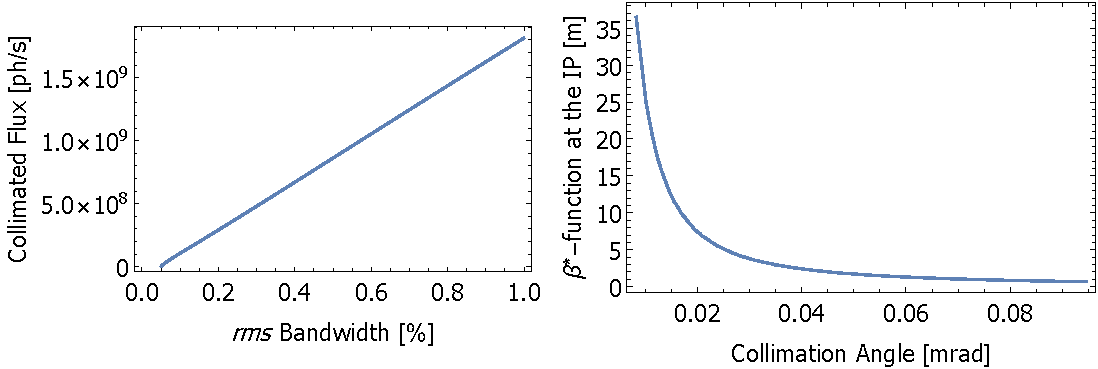
\includegraphics[width=\textwidth]{Figures/Optimisation_and_Characterisation_of_Inverse_Compton_Scattering_Sources/Case_A_RB_Tuning_Curves.pdf}
\caption{Case A (see Table~\ref{tab:char_opt_electron_bunch_parameters}) tuning curves in solution space ($\mathcal{F}_{\mathrm{col}}$--$\left(\Delta E_{\gamma}/E_{\gamma}\right)_{\mathrm{rms}}$) and parameter space ($\beta^{*}$--$\theta_{\mathrm{col}}$), using the round beam optimisation method in the narrowband regime ($\DeltaE_{\gamma}/E_{\gamma}/E_{\gamma}$). Left: Solution space plot showing the Pareto-optimal front. All solutions below the line are possible. Right: Parameter space plot showing the variable front corresponding to the Pareto-optimal front. Wide-band solutions favour large collimation angle and small $\beta$-function at the IP (collimation dominated), narrow-band solutions favour small collimation angle and and large $\beta$-function at the IP (emittance dominated). All solutions above the line are possible.}
\label{fig:CaseA_RB_tuning_curve}
\end{figure}

Fig.~\ref{fig:CaseA_RB_tuning_curve} shows the Pareto-optimal front (tuning curve) for the case A parameters within the \textit{rms} bandwidth range 0--1\%, the defined regime of narrowband operation. Small bandwidth limitation (Eq.~\ref{eq:bandwidth_limitation_minimum}) of $\sim$0.05\% exists due to the electron bunch energy spread and laser spectral bandwidth of the source. The collimated flux (Eq.~\ref{eq:collimated_flux}) appears to increase linearly with increasing \textit{rms} bandwidth.  

The case A $\beta^{*}$--$\theta_{\mathrm{col}}$ parameter space in Fig.~\ref{fig:CaseA_RB_tuning_curve} has a distinctive `elbow' shaped front corresponding to the Pareto-optimal front. All solutions above this front are possible and the front shown is optimal in the round beam case. Combinations of larger $\beta^{*}$-functions and collimation angles (and vice-versa) may have the same \textit{rms} bandwidth but will have reduced collimated flux. The most narrowband solutions have higher $\beta$-function at the IP and smaller collimation angle whereas the wider-band solutions exist at smaller $\beta$-functions at the IP and larger collimation angles. 

In the small collimation angle and large $\beta$-function region of the tuning curve $(\theta_{\mathrm{col}}< \sim0.02$~\si{\milli\radian}) the emittance term (Eq.~\ref{eq:emittance_term_round_beam}) dominates unlike in the wider-band, larger collimation angle and smaller $\beta^{*}$-function region ($\theta_\mathrm{col} > \sim0.02$~\si{\milli\radian}) where the collimation term dominates. A point exists in the tuning curve where emittance domination switches to collimation domination, which is not visible for case A but is visible in case C in Fig.~\ref{fig:case_C_optimisation_comparision}. 

\section{2D Non-Round Beam Optimisation}
\label{sec:NRB_optimisation}

In a non-round beam (NRB) optimisation the transverse normalised emittances ($\epsilon_{nx}/\epsilon_{ny}$) and the $\beta$-functions at the IP ($\beta_{x}^{*}/\beta_{y}^{*}$) in each plane can differ, as well as the collimation angle $\theta_{\mathrm{col}}$. Three variables are used in the optimisation, unlike the two in the RB optimisation method in Section~\ref{sec:RB_optimisation}. For a non-round beam optimisation, the selected $\beta$-function variables can not be easily bound or calculated as a function of each other as in (Eq.~\ref{eq:beta_star_maximum_limitation}) of the round beam methodology because the non-approximated emittance term (Eq.~\ref{eq:emittance_term}) is not simply re-arranged, unlike the emittance term in the RB case (Eq.~\ref{eq:emittance_term_round_beam}). Therefore, the non-round beam optimisation can't use the simple brute force optimisation method used in the RB optimisation in Section~\ref{sec:RB_optimisation}.

The NRB optimisation for a tuning curve (Pareto-optimal front) can be framed as a 3-dimensional, double objective non-linear minimisation problem of the form
\begin{align}
&\underset{\theta_{\mathrm{col}},~\beta_{x}^{*},~\beta_{y}^{*}}{\text{minimize}}, &-\mathcal{F}_{\mathrm{col}}\left(\theta_{\mathrm{col},~\beta_{x}^{*}},~\beta_{y}^{*}\right), \nonumber\\ 
& &\left(\frac{\Delta E_{\gamma}}{E_{\gamma}}\right)_{\mathrm{rms}}\left(\theta_{\mathrm{col}},~\beta_{x}^{*},~\beta_{y}^{*}\right), \nonumber\\
\nonumber\\
&\text{subject to} &0 \leq \theta_{\mathrm{col}} \leq \theta_{\mathrm{col,max}}, \nonumber\\
& &10^{-3}\leq \beta_{x}^{*} \leq\beta_{x,\mathrm{max}}^{*}, \nonumber\\
& &10^{-3}\leq \beta_{y}^{*} \leq\beta_{y,\mathrm{max}}^{*},
\label{eq:NRB_tuning_curve_optimisation_definition}
\end{align}
where $\mathcal{F}_{\mathrm{col}}$ is the collimated flux (Eq.~\ref{eq:collimated_flux}) and $\left(\Delta E_{\gamma}/E_{\gamma}\right)_{\mathrm{rms}}$ is the \textit{rms} bandwidth (Eq.~\ref{eq:RMS_bandwidth}) are the objective functions, $\theta_{\mathrm{col},\mathrm{max}}$ is the approximate upper bound on the collimation angle (Eq.~\ref{eq:collimation_angle_upper_bound}) and $\beta_{x/y,\mathrm{max}}^{*}$ are arbitrary upper bounds of the $\beta$-functions at the IP in each plane, set on a case by case basis. A minimum $\beta$-function at the IP  of $\beta_{x/y}^{*}=1$~\si{\milli\meter} is used as a reasonable limit of electron bunch final focus systems, discussed in Section~\ref{sec:objective_functions_and_variables}. The negative collimated flux objective function is minimised, therefore collimated flux is maximised.

For single point bandwidth optimisations, the problem is modified with a penalty function $\Omega$ (Eq.~\ref{eq:penalty_function}) instead of the \textit{rms} bandwidth (Eq.~\ref{eq:RMS_bandwidth}), and the problem becomes 
\begin{align}
&\underset{\theta_{\mathrm{col}},~\beta_{x}^{*},~\beta_{y}^{*}}{\text{minimize}}, &-\mathcal{F}_{\mathrm{col}}\left(\theta_{\mathrm{col},~\beta_{x}^{*}},~\beta_{y}^{*}\right), \nonumber\\ 
& &\Omega\left(\theta_{\mathrm{col}},~\beta_{x}^{*},~\beta_{y}^{*}\right), \nonumber\\
\nonumber\\
&\text{subject to} &0 \leq \theta_{\mathrm{col}} \leq \theta_{\mathrm{col,max}}, \nonumber\\
& &10^{-3}\leq \beta_{x}^{*} \leq\beta_{x,\mathrm{max}}^{*}, \nonumber\\
& &10^{-3}\leq \beta_{y}^{*} \leq\beta_{y,\mathrm{max}}^{*},
\label{eq:NRB_single_point_optimisation_definition}
\end{align}

Due to the complexity of the NRB optimisation problems, a more sophisticated approach to solving the optimisation problems than the RB case (Section~\ref{sec:RB_optimisation}) is required. Two optimisation methodologies are employed: a genetic algorithm (GA) approach, developed in collaboration with Prof B. Terzic, and a downhill simplex approach which are detailed in Sections~\ref{sec:genetic_algorithm_optimisation} and \ref{sec:simplex_optimisation}, then compared in Section~\ref{sec:evaluation_of_optimisation_methods}.

\subsection{Genetic Algorithm Approach}
\label{sec:genetic_algorithm_optimisation}
% Point heavily to SPEA2 paper etc.
% Just want to give an overview of how these things work
% Fitness, Mating, Strength etc. -> what happens?
% define feasible, non-dominated, individual, generation etc.
In a genetic algorithm, a set of individuals -- a single point in multi-dimensional parameter space -- known as a population are randomly generated in the bounded parameter space; all of these points are feasible solutions to the optimisation problem. The objective functions are then calculated for each individual based on these variables and a fitness function, dependent on the objective functions, that measures how well an individual meets the optimization goals \cite{hofler2013innovative} is then evaluated. The design of fitness functions vary greatly between different genetic algorithms. The individuals are then evaluated against each other via a competition -- typically a head-to-head fitness comparison between pairs of individuals -- where the fitter (higher fitness) individuals that triumph over other individuals are selected to form a subset named the mating pool. The mating pool is the set of individuals which dominate (triumph over) other individuals in the population and aren't dominated by any other individual -- they are non-dominated. The mating pool individuals are the subset of the population which will form the next generation, which is the new population of the next iteration. In most GA's some non-dominated points of the previous generation are also inducted into the next generation. Individuals in the mating pool are paired together (randomly or otherwise) and through recombination, the exchange of variable values, and mutation, adjustment (scaling) of single parameter space variables \cite{hofler2013innovative} -- designed to mimic biological reproduction -- a set of new individuals for the next generation, named offspring, are produced.

Therefore, a genetic algorithm operates with a general basic procedure to solve a multi-dimensional multi-objective optimisation problem:
\begin{enumerate}
    \item{A population of individuals are randomly generated to sample the parameter space.}
    \item{Objective and fitness functions are evaluated for each individual in the new generation}
    \item{All non-dominated individuals of the previous generation are introduced (step doesn't apply in generation 1). }
    \item{If a termination condition is met, for example the no. generations exceeds a pre-set value, the simulation stops and the non-dominated individuals make up the Pareto front. }
    \item{A form of competition is used to select candidates to form the mating pool, which decides the composition of individuals in the next generation.}
    \item{Individuals in the mating pool are paired together (randomly or otherwise) and these produce the individuals of the next generation via recombination and mutation}
    \item{A new generation begins. The simulation is iterated starting from step 2. This repeats until the termination condition in step 4 is satisfied.}
\end{enumerate}
Once the termination condition has been satisfied, the Pareto-optimal front is produced and the parameters of all of the non-dominated individuals that constructed the Pareto-optimal front are returned. 

The genetic algorithm (GA) optimisation uses the minimisation routine of \textsc{SPEA2} \cite{zitzler2001spea2} within the \textsc{PISA} platform \cite{bleuler2003pisa} framework, following the methodology outlined by A. Hofler et al \cite{hofler2013innovative}. The \textsc{SPEA2} algorithm is a multi-objective evolutionary algorithm which incorporates a fine grained fitness assignment strategy \cite{zitzler2001spea2} with density evaluation, using an archive of non-dominated points from previous generations to supplement determination of the mating pool of the current generation. In the \textsc{SPEA2} algorithm, the fitness function is defined by
\begin{itemize}
    \item{Assigning each individual a strength value representative of the number of solutions it dominates.}
    \item{Defining raw fitness based upon the strength value of the current population and archived population.}
    \item{Calculating a density function for each individual, using the $k$th nearest neighbour method \cite{silverman1986density}, which is introduced as raw fitness can fail when most individuals don't dominate eachother for example, when there are many objectives.}
    \item{The fitness is then defined as the raw fitness plus the density.}
\end{itemize}
A full explanation of the fitness determination is omitted for brevity, and is better described by Zitzler et al \cite{zitzler2001spea2}. The \textsc{SPEA2} fitness function enables the non-dominated Pareto-optimal set to be determined efficiently and reliably.

The developed GA utilises a set of \textsc{Python} scripts designed to calculate the objective functions ($\mathcal{F}_{\mathrm{col}}$, $\left(\Delta E_{\gamma}/E_{\gamma}\right)_{\mathrm{rms}}$) which are implemented on the \textsc{PISA} platform \cite{bleuler2003pisa}, configured for three variables and two objective functions. The algorithm is generalised for simulation of any linear ($a_{0} \ll 1$) ICS source. Upper and lower limits of the variables are imposed as mentioned in (Eqs.~\ref{eq:NRB_tuning_curve_optimisation_definition}, \ref{eq:NRB_single_point_optimisation_definition}) with  $\beta_{x/y}^{*}\sim 10$'s~\si{\meter}. Multiple equally valid solutions exist in the solution space, as this is a global optimisation, defining a Pareto-optimal front. Each solution on the Pareto-optimal front is a feasible solution, non-dominated with respect to other individuals that contribute to the Pareto front and dominates another feasible individual in the solution space \cite{hofler2013innovative}. The Pareto-front non-dominated individual parameters (variable and objective function values) are wrote to file as well as all parameters of the individuals trialed within the course of the optimisation.  

Optimisation settings for the GA NRB optimisation are the standard configuration used in \textsc{SPEA2}, for further explanation of these parameters see Zitzler et al \cite{zitzler2001spea2}. Preliminary studies showed negligible variation in the solution through variation of these, except for the termination conditions (number of generations) and the population size. The optimisation terminates after 200 generations and 50 individuals are used because preliminary studies showed this was a good balance between optimisation time and coverage of the parameter space. Full benchmarking of each simulation setting for a GA is extensive and, for the method chosen here, is beyond the scope of the initial work. 

The tuning curve mapping the optimised configurations of the ICS source is the Pareto-optimal front defined in solution space, as the Pareto-optimal front consists of the maximal collimated flux for each \textit{rms} bandwidth constrained by the variable limits. Whereas, in the single point optimisations, a Pareto-optimal front of the collimated flux as a function of the penalty function is returned. The single optimal solution is decided in a post-processing selection procedure where all values that fit the penalty function criteria of $\Omega < 10^{-5}$, used as this is well below experimental tolerances, are compared and the solution with the maximal collimated flux is chosen. This selection procedure is advantageous over choosing the point with the minimum penalty function because anomalous points near $\Omega = 0$, with reduced collimation flux can occur due to a lack of individuals achieving a small penalty function.          

The genetic algorithm method is a global optimisation technique providing a set of solutions for each optimisation run -- not just a single solution -- allowing the full solution space ($\mathcal{F}_{\mathrm{col}}$--$\left(\Delta E_{\gamma}/E_{\gamma}\right)_{\mathrm{rms}}$) to be mapped more effectively. Consequently, optimisation via a GA delivers a global maximum for the collimated flux at each of the \textit{rms} bandwidths or values of the penalty function, within the limits of the variables, unlike in local optimisation where the optimisation may become stuck in a local minima. By inspection of the variables in parameter space corresponding to the non-dominated Pareto-optimal individuals in solution space, relationships can be deduced. Characteristics of the Pareto-optimal variables parameter space, such as stratification of the individual shows some variables affect the objective functions more than others. For example, a lesser spread in the Pareto-optimal variable vales of $\theta_{\mathrm{col}}$ compared to $\beta_{x}^{*}$ would suggest that $\theta_{\mathrm{col}}$ is a more important variable to the optimisation. However, if the parameter space is simple the GA method may be overly sophisticated for the problem and less complicated optimisation may be similarly accurate and precise. Further benchmarking of simulation parameters such as the mutation probability etc. is required as investigations have been limited, yielding negligible variation. Termination conditions must also be further optimised. 

The genetic algorithm approach has been applied to the electron bunch benchmarking case A in Table~\ref{tab:char_opt_electron_bunch_parameters} using the laser parameters in Table~\ref{tab:char_opt_laser_pulse_parameters} with a population of 50 individuals and a total of 200 generations. The tuning curves (parameter and variable space) produced via the genetic algorithm method for case A in the narrowband range ($\Delta E_{\gamma}/E_{\gamma}<1\%$) are shown in Fig.~\ref{fig:case_A_GA_tuning_curves} demonstrating the typical output of the NRB genetic algorithm, where both the non-dominated Pareto front points and the other trial points are shown. Onward from this section in the thesis only the Pareto front points and their corresponding variables will be included in plots to aid comparison of optimisation methods. GA optimisations for case B and C are shown in comparative plots in Figs.~\ref{fig:case_B_optimisation_comparison)}, \ref{fig:case_C_optimisation_comparision} but not shown here for brevity. 
\begin{figure}[!h]
\centering
\includegraphics[width=\textwidth]{Figures/Optimisation_and_Characterisation_of_Inverse_Compton_Scattering_Sources/CaseA_GA_Tuning_Curve.pdf}
\caption{Case A genetic algorithm tuning curves (solution and parameter space) produced using 200 generations and 50 individuals, showing the non-dominated Pareto front points (red) and the dominated trial points (blue). Top Left: collimated flux as a function of \textit{rms} bandwidth solution space. Top Right: parameter space plot of the $\beta$-function in the $x$ plane as a function of the $\beta$-function in the $y$ plane at the IP. Bottom Left: parameter space plot of the $\beta_{x}$-function at the IP as a function of the collimation angle. Bottom Right: parameter space plot of the $\beta_{y}$-function at the IP as a function of the collimation angle.}
\label{fig:case_A_GA_tuning_curves}
\end{figure}

In Fig.~\ref{fig:case_A_GA_tuning_curves}, a well defined Pareto-optimal front in the collimated flux--\textit{rms} bandwidth solution space is visible. The individuals in the solution space Pareto-optimal front are clearly non-dominated, with a series of dominated points shown below this front. The resulting Pareto-optimal front is the maximal collimated flux as a function if \textit{rms} bandwidth, and therefore a tuning curve for the case A ICS source. There is also a minimum \textit{rms} bandwidth cut-off at $\sim 0.1$\%, as predicted by Eq.~\ref{eq:bandwidth_limitation_minimum}. A maximum collimated flux of $\sim 1.9\times 10^{9}$~ph/\si{\second} is expected at 1\% \textit{rms} bandwidth.

The $\beta_{x}^{*}$--$\beta_{y}^{*}$ parameter space plot shows that the variables corresponding to the non-dominated solutions do not follow the round beam solution ($\beta_{x}^{*}\neq\beta_{y}^{*}$). Therefore, the round beam solution is sub-optimal and non-round beam simulation is beneficial even when the transverse emittance of the electron beam is round ($\epsilon_{nx}=\epsilon_{ny}=\epsilon_{n}$). Typically, the Pareto-optimal variables favour $\beta_{x}^{*}>\beta_{y}^{*}$ because the crossing angle is imposed in the $x$--$z$ plane; this is the only difference between the two transverse planes. When $\beta_{x}^{*}>10$~\si{\meter} the spread of the optimal $\beta$-functions at the IP becomes large because the parameter space is highly constrained; these correspond to solutions for the narrowest bandwidths. Many dominated individuals exist around the parameter space of the Pareto-optimal individuals in the $\beta_{x}^{*}$--$\beta_{y}^{*}$ parameter space, demonstrating that the parameter space is well explored.

The parameter spaces  of the $\beta$-functions against the collimation angle differ in each plane due to the crossing angle in the $x$--$z$ plane, but both show a characteristic `elbow' shape. The $\beta_{x}$--$\theta_{\mathrm{col}}$ parameter space shows a large stratification in the Pareto-optimal variable positions which shows the objective functions have a weak dependence on this variable, this plot varies largely from the $\beta^{*}$--$\theta_{\mathrm{col}}$ parameter space curve in Fig.~\ref{fig:CaseA_RB_tuning_curve}. In comparison, the $\beta_{y}^{*}$--$\theta_{\mathrm{col}}$ parameter space plot shows far less stratification of the Pareto-optimal front variables and a clearer `elbow' shape of the optimal variables, also present in the parameter space of the RB optimisation in Fig.~\ref{fig:CaseA_RB_tuning_curve}. In both of the $\beta$-function at the IP against collimation angle parameter space plots for case A there appears to be a lack of statistics -- dominated points -- around 0.02~\si{\milli\radian}, the cause of which is unknown though this may be a random occurrence in the optimisation.    

\subsection{Simplex Approach}
\label{sec:simplex_optimisation}

The downhill simplex method is a direct search optimisation method used to minimise a set of objective functions. It is a local optimisation method, used to find a global solution to the collimated flux (Eq.~\ref{eq:collimated_flux})--\textit{rms} bandwidth (Eq.~\ref{eq:}) trade-off. A global solution is possible from local optimisation methods if the parameter space of the optimisation problem (Eq.~\ref{eq:NRB_single_point_optimisation_definition}) is not complex, else a local minima solution will be achieved. In this section the simplex methodology is outlined, its application to the optimsation problem for the single point bandwidth (Eq.~\ref{eq:NRB_single_point_optimisation_definition}) is explained, and extension to the tuning curve case is demonstrated. The simplex method will be explained using the \textsc{Mathematica} formalism \cite{wolfram2021nmaximize}, as \textsc{Mathematica}'s \textsc{NMaximise} function is used for the NRB optimisation.

In downhill (minimisation) simplex optimisation, for an optimisation problem with $n$ variables, a set of $n+1$ points ($x_{1}$--$x_{n+1}$) are used to form the vertices of a polytope in an $n$-dimensional parameter space \cite{wolfram2021nmaximize} . For example, in the NRB optimisation (Eq.~\ref{eq:NRB_tuning_curve_optimisation_definition}) there are three variables so the polytope is a 4-vertex polyhedron in parameter space. Selection of the vertex points can be prescribed, but random selection allows the potential to fully investigate the parameter space \cite{koshel2002enhancement}. The objective function $f\left(x\right)$ is calculated for each of these vertex's and they are sorted into the form
\begin{equation}
f\left(x_{1}\right) \leq f\left(x_{2}\right) \leq \ldots \leq f\left(x_{n+1}\right),
\label{eq:simplex_polytope_objective_functions}
\end{equation}
where the objective functions are ordered from minimum objective function ($x_{1}$, best point) to maximum objective function ($x_{n+1}$, worst point). The worst point is then replaced by a trial point $x_{t}$, given by
\begin{equation}
x_{t} = c+s_{r}\left(c-x_{n+1}\right),
\label{eq:simplex_trial_point}    
\end{equation}
which denotes a reflection of the worst point $x_{n+1}$, with $s_{r} > 0$ the refection parameter, and the midpoint $c$ of the $n$-dimensional polytope is given by
\begin{equation}
c = \frac{1}{n}\sum_{i=1}^{n}x_{i}.
\label{eq:polytope_centroid_simplex}
\end{equation}
If $x_{t}$ minimises the objective better than the best point ($f\left(x_{t}\right) \leq f\left(x_{1}\right)$), then reflection is a successful objective function minimisation method. The polytope is then expanded in the reflected direction because this could provide further minimisation of the objective function. The new trial point $x_{e}$ is given by
\begin{equation}
x_{e} = c+s_{e}\left(x_{t}-c\right),
\label{eq:simplex_expansion}    
\end{equation}
where $s_{e} > 1$ is the expansion parameter. If $f\left(x_{e}\right) < f\left(x_{t}\right)$, $x_{e}$ is a better solution and replaces the worst point in the set $x_{n+1}$, otherwise $x_{t}$ replaces $x_{n+1}$. 

Contraction of the polytope could provide a better solution if the new trial point $x_{t}$ is worse than the the second worst point $f\left(x_{t}\right) \geq f\left(x_{n}\right)$, the new trial vertex becomes
\begin{equation}
x_{c} = 
\begin{cases}
c+s_{c}\left(x_{n+1}-c\right), & \text{if}  ~f\left(x_{t}\right) \geq f\left(x_{n+1}\right), \\
c+s_{c}\left(x_{t}-c\right), & \text{if}  ~f\left(x_{t}\right) < f\left(x_{n+1}\right),
\end{cases}
\label{eq:simplex_contraction}
\end{equation}
where $0 < s_{c} < 1$ is the contraction parameter. A further contraction, named a shrink, is carried out if $f\left(x_{c}\right) < f\left(x_{n+1}\right) \land f\left(x_{t}\right)$ because the previous contraction was successful, with $x_{t}$ replacing $x_{n+1}$. A shrink would be of identical form to (Eq.~\ref{eq:simplex_contraction}) with the contraction parameter $s_{c}$ replaced by a shrink parameter $0 < s_{s} < 1$. The method is then iterated until the termination condition -- typically a number of iterations -- is exceeded or until convergence below a set tolerance in the penalty function (Eq.~\ref{eq:penalty_function}) is achieved. 

To introduce constraints into the simplex optimisation a penalty function can be used to test the $n$-dimensional polytope vertices against the constraints using a penalty function, as outlined by Myers and Carter \cite{myers1973response}. For example, if the constraints of (Eq.~\ref{eq:NRB_single_point_optimisation_definition}) are violated by polytope vertex then the objective function could be set to some large number so it is not selected for further optimisation. Multi-objective optimisation -- since we have minimised an \textit{rms} bandwidth penalty function (Eq.~\ref{eq:penalty_function}) and maximised collimated flux (Eq.~\ref{eq:collimated_flux}) objectives -- is implemented using the $\epsilon$-Constraint method \cite{marler2004survey}, where the bandwidth penalty function (Eq.~\ref{eq:penalty_function}) is re-cast into a constraint where $\Omega < \epsilon$, and $\epsilon$ is a small tolerance of $\epsilon = 10^{-5}$, as used in Section~\ref{sec:genetic_algorithm_optimisation}.  

The simplex optimisation is typically quick because a minimum of $n+1$  objective function calculations, with $n$ variables, are required per iteration in comparison to genetic algorithm methods where objective functions are calculated for each individual. Since a single trial point is compared against $n+1$ points in each iteration, the comparative aspect of a downhill simplex method is also more efficient. Therefore, downhill simplex optimisation can be completed on the minute-scale for the single point optimisation examples. A full benchmarking of the simplex method is also more readily achievable due to the small number of simulation settings that can be adjusted -- these consist of the 4 constants governing refection and expansion etc., the tolerance of the simulation and the no. iterations.   

The downhill simplex optimisation method is a local minimisation routine as derivatives are effectively used to find minima \cite{jones2016design}. Therefore, unlike in the GA method, only a single solution space point is returned for each optimisation and the full solution space is not mapped in this optimisation. As a heuristic method, simplex optimisation may fail to find the global optimal solution and become trapped in a local minima, though in practice downhill simplex is efficient in finding global minima where few local minima exist in the parameter space \cite{wolfram2021nmaximize}. The parameter space of the NRB optimisation problem (Eq.~\ref{eq:NRB_tuning_curve_optimisation_definition}) is assumed to be simple enough to produce a global minima result, however this assumption will be evaluated in Section~\ref{sec:evaluation_of_optimisation_methods} by comparison with the GA NRB method. Another limitation of this method is that the optimisation arbitrarily terminates after a set number of iterations, which may mean that a true optimal solution is not found if finding it exceeds the iteration limit.

The optimisation uses the \textsc{NMaximise} maximisation routine in \textsc{Mathematica} \cite{wolfram2021nmaximize} where the collimated flux (Eq.~\ref{eq:collimated_flux}) objective function is maximised and the bandwidth penalty function (Eq.~\ref{eq:penalty_function}) is minimised using the $\epsilon$-constraint method discussed above. In order to produce tuning curves using the simplex method, the optimisation is applied to an array of 200 bandwidth values, as for the RB optimisation in Section~\ref{sec:RB_optimisation}. The interaction point $\beta$-functions and collimation angle are initialised as variables, therefore the optimisation problem is stated as in (Eq.~\ref{eq:NRB_single_point_optimisation_definition}) with the collimation upper bound given by (Eq.~\ref{eq:collimation_angle_upper_bound}) and maximum $\beta$-functions at the IP arbitrarily set on a case by case basis. A maximum of 200 iterations are used. Default values of the ReflectRatio ($s_{r}$), ExpandRatio ($s_{e}$), ContractRatio ($s_{c}$) and ShrinkRatio ($s_{s}$) parameters \cite{wolfram2021nmaximize}, corresponding to the coefficients in (Eqs.~\ref{eq:simplex_trial_point}--\ref{eq:simplex_contraction}), are used as they are sufficient to optimise all of the cases in Table~\ref{tab:char_opt_electron_bunch_parameters}.

The results of the simplex NRB tuning curve optimisations for benchmarking case A are shown in Fig.~\ref{fig:case_A_simplex_tuning_curves} for the narrowband ($\Delta E_{\gamma}/E_{\gamma} \leq1$\%) regime. The $\beta$-functions at the IP are upper bounded by $\beta_{x/y}^{*} < 20~\mathrm{\si{\meter}}$ and tuning curves are produced using 200 iterations and the \textsc{Mathematica} \cite{wolfram2021nmaximize} default values of the simplex scaling parameters ($s_{r}$, $s_{e}$, $s_{c}$, $s_{s}$). 
\begin{figure}[!h]
\centering
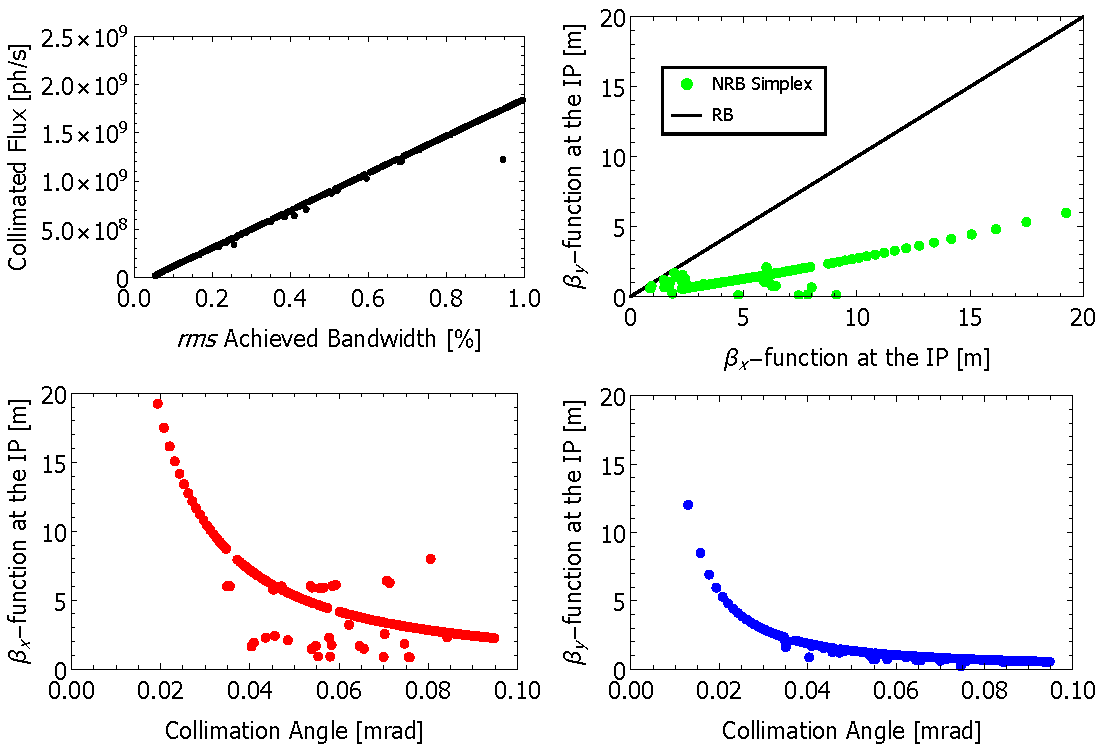
\includegraphics[width=\textwidth]{Figures/Optimisation_and_Characterisation_of_Inverse_Compton_Scattering_Sources/Case_A_simplex_Tuning_Curves.pdf}
\caption{Case A simplex optimisation tuning curves in both solution and parameter space. Top Left: Pareto-optimal front of the collimated flux as a function of \textit{rms} bandwidth. Top Right: Simplex parameter space ($\beta_{x}^{*}$--$\beta_{y}^{*}$) variable front (green) corresponding to the Pareto-optimal front in solution space compared to the monotonically varying round beam variable front (black). Bottom Left: Parameter space ($\beta_{x}^{*}$--$\theta_{\mathrm{col}}$) corresponding to the Pareto-optimal front in solution space. Bottom Right: Parameter space ($\beta_{y}^{*}$--$\theta_{\mathrm{col}}$) corresponding to the Pareto-optimal front in solution space.}
\label{fig:case_A_simplex_tuning_curves}
\end{figure}

The Pareto-optimal front in solution space ($\mathcal{F}_{\mathrm{col}}$--$\left(\Delta E_{\gamma}/E_{\gamma}\right)_{\mathrm{rms}}$) in Fig.~\ref{fig:case_A_simplex_tuning_curves} is well defined in the 0--1\% \textit{rms} bandwidth range. The minimum achieved bandwidth is around $\sim0.1$\%, as expected using (Eq.~\ref{eq:bandwidth_limitation_minimum}). A maximum collimated flux of $\sim 1.9\times 10^{9}$~ph/\si{\second} in a 1\% \textit{rms} bandwidth is predicted, identical to Fig.~\ref{fig:case_A_GA_tuning_curves}. Convergence to local minima solutions appears to occur for few points in solution space; the complexity of solution space is minimal, and the downhill simplex method is generally satisfactory for case A.  

The $\beta_{x}^{*}$--$\beta_{y}^{*}$ parameter space plot corresponding to the tuning curve in solution space shows that the optimal solution is a non-round transverse electron bunch profile at the IP because The $\beta_{x}^{*}$-function is typically larger than the $\beta_{y}^{*}$ function in Fig.~\ref{fig:case_A_simplex_tuning_curves}. A larger horizontal spot size is favoured because of the non-zero crossing angle between the electron bunch and laser pulse in the $x$--$z$ plane. Both the $\beta$-function at the IP against collimation angle parameter space plots display the typical `elbow' shape observed in the RB case in Fig.~\ref{fig:CaseA_RB_tuning_curve}. However, the $\beta_{x}^{*}$--$\theta_{\mathrm{col}}$ plot contains numerous off-trend Pareto-front corresponding points in local minima, which lay in the range $0.03~\textrm{\si{\milli\radian}} < \theta_{\mathrm{col}} < 0.09~\mathrm{\si{\milli\radian}}$. More local minima in $\beta_{x}^{*}$ suggests the $\beta_{x}^{*}$ variable has a weak dependence on collimated flux. However, the parameter space plot shows that the quantity of local minima in simplex NRB optimisation is small and, by checking single point optimisations against wider range tuning curves, local minima can be readily identified.

\section{Evaluation of Optimisation Methods} 
\label{sec:evaluation_of_optimisation_methods}

Optimisations have been performed for each of the cases in Table~\ref{tab:char_opt_electron_bunch_parameters} using the laser parameters in Table~\ref{tab:char_opt_laser_pulse_parameters} using the RB (Section~\ref{sec:RB_optimisation}), GA NRB and simplex NRB (Section~\ref{sec:NRB_optimisation} methods. Since case B electron bunch parameters don't fulfill the round beam optimisation criteria ($\epsilon_{nx}\neq\epsilon_{ny}$) it has been excluded from the RB method. Within this section, the optimisation methods will be compared through both single point and tuning curve optimisations, to evaluate the applicability of optimisation towards narrowband radiation production, quantify the advantage of NRB optimisation over RB optimisation and examine the feasibility of each optimisation method. 

Applying these optimisation techniques in practice requires further studies. For example, accelerator jitter may impede the the optimised electron bunch transverse profile at the interaction point from being produced and the effect of this error on source performance needs to be quantified. Errors such as misalignment of the incident laser pulse and collimator must also be studied. This is a subject for future work.  

\subsection{Single Point Bandwidth Optimisations}

Single point bandwidth optimisations of the benchmarking cases in Table~\ref{tab:char_opt_electron_bunch_parameters}, with laser parameters in Table~\ref{tab:char_opt_laser_pulse_parameters}, are used to compare optimisation methods (RB, NRB simplex and NRB GA) at small \textit{rms} bandwidths (0.5\% \texit{rms} bandwidth for case A and C and 2\% \texit{rms} bandwidth for case B) to quantify the advantage of using each method and for comparison against the standard transverse profile matching approach in Section~\ref{sec:transverse_profile_matching}. The single point bandwidth optimised results of each case are shown in Table~\ref{tab:single_point_optimisations}. 

Comparison between optimisation methods will determine if optimising the transverse dynamics for maximal collimated flux in a narrow bandwidth is a worthwhile strategy and ascertain the benefit of using a non-round beam optimisation, beyond the obvious advantage that RB optimisation is only applicable when certain criteria are satisfied. Through examination of the variables related to the optimal solution, ICS source design can be further understood and the question of whether a round transverse profile is optimal can be answered.      

\begin{table}[!h]
\centering
\caption{Single point optimisations for the transverse profile matching (TPM), round beam (RB), non-round beam simplex (NRB simplex) and non-round beam genetic algorithm (NRB GA) methods of all benchmarking cases. \textit{Rms} bandwidths of 0.5\% (2\%) are chosen to evaluate the single point optimisation methodologies for case A and C (case B). The optimisations are compared via the collimated flux, which is maximised, and the variables corresponding to the optimal solution.}
\vspace{3mm}
\begin{threeparttable}
\begin{tabular}{lccccc}
\hline\hline
Parameter & TPM & RB & NRB simplex & NRB GA & Unit \\
\hline
\multicolumn{6}{c}{Case A 0.5\% \textit{rms} bandwidth} \\
\hline
Collimated flux & $7.37\times 10^{8}$ & $8.62\times 10^{8}$ & $8.81\times 10^{8}$ & $8.86\times 10^{8}$ & ph/\si{\second} \\
$\beta_{x}^{*}$-function & 3.53 & 1.15 & 1.69 & 2.11 & \si{\meter}\\
$\beta_{y}^{*}$-function & 3.53 & 1.15 & 0.88 & 0.87 & \si{\meter}\\
Collimation angle & 0.068 & 0.066 & 0.066 & 0.066 & \si{\milli\radian}\\
\hline
\multicolumn{6}{c}{Case B 2\% \textit{rms} bandwidth} \\
\hline
Collimated flux & -- & -- & $9.19\times 10^{9}$ & $1.04\times 10^{10}$ & ph/\si{\second} \\
$\beta_{x}^{*}$-function & -- & -- & 3.46 & 11.05 & \si{\meter} \\
$\beta_{y}^{*}$-function & -- & -- & 0.10 & 0.20 & \si{\meter} \\
Collimation angle & -- & -- & 0.178 & 0.194 & \si{\milli\radian} \\ 
\hline
\multicolumn{6}{c}{Case C 0.5\% \textit{rms} bandwidth} \\
\hline
Collimated flux & $8.35\times 10^{7}$ & $1.16\times 10^{8}$ & $1.16\times 10^{8}$ & $1.17\times 10^{8}$ & ph/\si{\second} \\
$\beta_{x}^{*}$-function & 0.45 & 0.015 & 0.016 & 0.029 & \si{\meter} \\
$\beta_{y}^{*}$-function & 0.45 & 0.015 & 0.015 & 0.013 & \si{\meter} \\
Collimation angle & 2.63 & 2.62 & 2.63 & 2.64 & \si{\milli\radian}\\
\hline\hline
\end{tabular}
\begin{tablenotes}
\item[*]{Transverse profile matching settings aren't possible because the emittance term (Eq.~\ref{eq:emittance_term}) for $\sigma_{\mathrm{electron}} = \sigma_{L}$ leads to a larger than 2\% \textit{rms} bandwidth.}
\item[$\dagger$]{This case doesn't satisfy the round beam condition ($\epsilon_{nx} \neq \epsilon_{ny}$), therefore the RB optimisation can't be utilised.}
\end{tablenotes}
\end{threeparttable}
\label{tab:single_point_optimisations}
\end{table}

Comparing the collimated flux for case A in Table~\ref{tab:single_point_optimisations}, the collimated flux in the transverse profile matching case is exceeded by all optimised cases, with a 17.0\% increase in collimated flux from the RB optimisation and a 20.2\% increase in collimated flux from the GA NRB optimisation, with respect to the transverse profile matching case. There is a small 2.8\% increase in collimated flux of using a GA NRB optimisation in comparison to a RB optimisation, however a small increase expected as the optimised case A adheres to the round beam criteria well ($\epsilon_{nx}=\epsilon_{ny}=\epsilon_{n}$, $\beta_{x}^{*}\sim\beta_{y}^{*}$). The collimated flux advantage in the NRB method must result from the angular crossing luminosity reduction term (Eq.~\ref{eq:angular_crossing_factor}) because each transverse plane of the interaction is otherwise identical. The $\beta$-functions in each plane of this case differ, therefore the optimal transverse profile of the electron bunch is not round. The simplex NRB case produces a reduced collimated flux in comparison to the GA method; the variation in the solutions is observed in the $\beta_{x}^{*}$ variables, however there is also a negligible difference in collimation angle. 

Single point optimisation results for case B, in Table~\ref{tab:single_point_optimisations}, show both the transverse profile matching method and round beam optimisation could not be used. The transverse profile matching method leads to a large emittance term (Eq.~\ref{eq:emittance_term}) in the bandwidth, which means a \textit{rms} bandwidth of 2\% can't be achieved -- in fact an \textit{rms} bandwidth below $\sim$20\% is not achievable. The round beam optimisation is, as aforementioned, unsuitable due to the mismatched emittances in each plane ($\epsilon_{nx}\neq\epsilon_{ny}$). Comparison of the collimated flux of the GA NRB case to the simplex NRB case shows a collimated flux increase of 13.2\% by using the GA method. The large discrepancy between NRB optimisations may be evidence of the simplex method encountering a local minima; mismatched emittances ($\epsilon_{nx}\neq\epsilon_{ny}$) may complicate the solution space. The variability in NRB optimisation is much larger in case B than the other cases. Furthermore, there is a large discrepancy in the $\beta_{x}^{*}$ function at the IP, with the simplex method yielding a $\beta_{x}^{*}$ function $\sim3$ times lower than in the GA method with similar factor of 2 discrepancies in $\beta_{y}^{*}$ and a 8.9\% increase in the collimation angle with respect to the downhill simplex method. The transverse profile of the electron bunch in this case is highly asymmetric, for example for the GA NRB optimisation $\sigma_{\mathrm{electron},x} = 389.2$~\si{\micro\meter} and $\sigma_{\mathrm{electron},y} = 5.8$~\si{\micro\meter}.

For case C, Table~\ref{tab:single_point_optimisations} shows that 38.9\% and 40.1\% increases in collimated flux are achieved via using the round beam and GA non-round beam optimisation methods respectively over transverse profile matching -- a significant improvement. However, comparing the NRB solutions with the RB solution, no notable increase in collimated flux is achieved. The NRB optimisations have provided similar collimated flux to the RB optimisation because case C fits the round beam criteria particularly well; the emittance is very small, identical in each plane and the short bunch length suppresses the crossing angle effect where the $\beta_{x}^{*} > \beta_{y}^{*}$ bias is introduced. Very modest asymmetry in the transverse profile of the electron bunch in the case C GA NRB optimisation is observed, which reinforces the case A conclusion that a round electron bunch transverse profile in not optimal.      

To summarise, in Table~\ref{tab:single_point_optimisations} the GA NRB single point bandwidth optimisation method consistently provides the most optimal solution, though the simulation time is much longer: $t_{\mathrm{sim}}\approx 5$~\si{\minute} for simplex NRB optimisation compared with $t_{\mathrm{sim}}\approx 50$~\si{minute} for GA NRB optimisation. Though reduction of the 200 generation termination condition could reduce the time of the GA method, whilst reducing optimisation precision. The NRB optimisation method is found to be necessary in cases where the emittances are mismatched and therefore it is especially valuable for storage ring driven ICS sources because ERL and linac drivers conform more readily to the RB criteria. Case A and C showed that optimisation provided on the order of 10's\% more collimated flux than the transverse profile matching scheme, therefore optimisation is necessary for high flux, narrowband ICS based light source operation. The optimal transverse profiles of all the trialed cases in Table~\ref{tab:single_point_optimisations} are asymmetric, so NRB optimisation can be worthwhile when emittances are identical in each plane. The downhill simplex method may potential encounter local minima, as potentially observed in case B simplex NRB optimisation. The most obvious solution to the problem of local minima is to combine the simplex optimiser with a non-derivative-based heuristic optimisation method \cite{jones2016design}, therefore combining a limited (by no. generations) GA NRB method to find a global solution with a downhill simplex method to quickly fine tune the optimisation may be the best method of optimisation. A combined GA and downhill simplex method would be a suitable investigation for further study.

\subsection{Tuning Curve Optimisations}

Comparison of tuning curve optimisations via differing methods for the three test cases in Table~\ref{tab:char_opt_electron_bunch_parameters} allows evaluation of the optimisation methods efficacy at mapping out the capabilities of an ICS source. Comparison of different ICS sources would also be furthered by comparison of their tuning curves, not just single configurations, as is best practice in other light source facilities such as synchrotron light sources and free electron lasers. Solution and parameter space tuning curves, such as those in Figs.~\ref{fig:}, would also enable ICS source users to find optimal configurations for experiments. 

A comparison of the tuning curve optimisation methods for the case A parameters in Table~\ref{tab:char_opt_electron_bunch_parameters} is shown in Fig.~\ref{fig:case_A_optimisation_comparison}. The case A solution space tuning curve ($\mathcal{F}_{\mathrm{col}}$--$\left(\Delta E_{\gamma}/E_{\gamma}\right)_{\mathrm{rms}}$) shows a small increase in collimated flux for the NRB solutions in comparison to the RB method, the difference in collimated flux between these methods increases with a wider bandwidth. As expected, the minimum achievable bandwidth (Eq.~\ref{eq:bandwidth_limitation_minimum}) of each of the tuning curves produced by the three methods agrees as this is limited by the energy spread of the electron bunch and laser pulse spectral bandwidth.

\begin{figure}[!h]
\centering
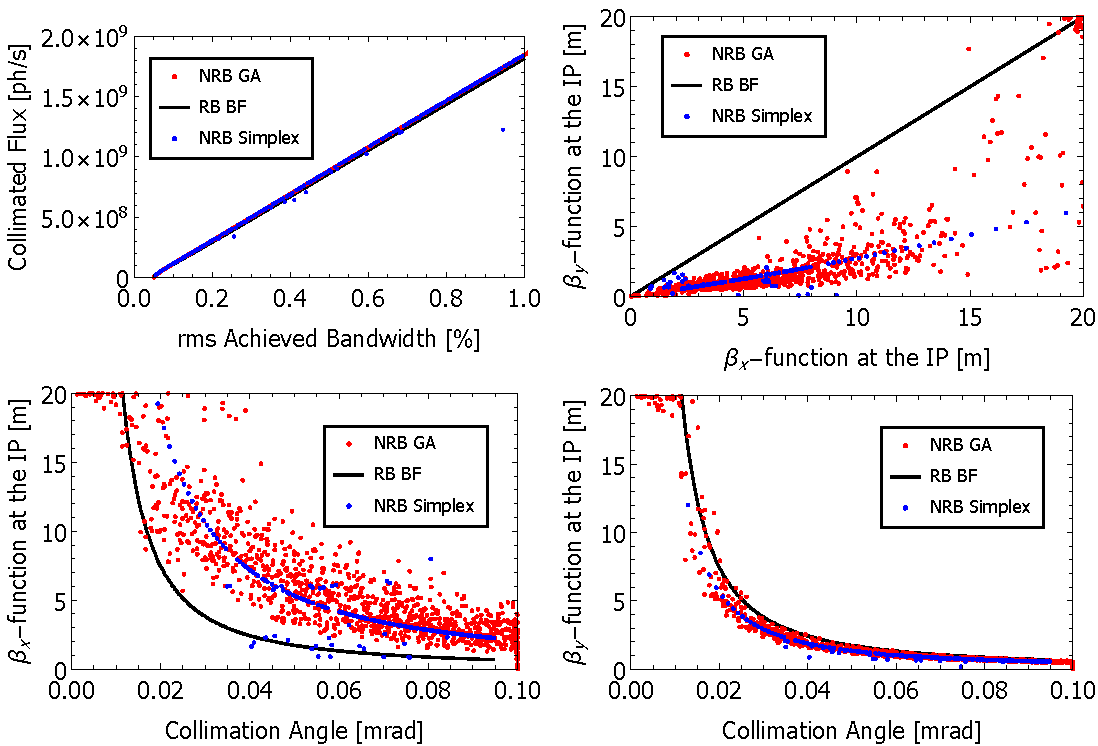
\includegraphics[width=\textwidth]{Figures/Optimisation_and_Characterisation_of_Inverse_Compton_Scattering_Sources/CaseAoptcomp.pdf}
\caption{Comparison of the three optimisation methods: RB (black), GA NRB (red) and simplex NRB (blue), used in maximal collimated flux narrowband ICS optimisation for the case A parameters (see Table~\ref{tab:char_opt_electron_bunch_parameters}). $\beta$-functions at the IP in each plane and collimation angle are varied. Top Left: Solution space ($\mathcal{F}_{\mathrm{col}}$--$\left(\Delta E_{\gamma}/E_{\gamma}\right)_{\mathrm{rms}}$) Pareto-optimal fronts. Top Right: Parameter space ($\beta_{x}^{*}$--$\beta_{y}^{*}$) variable fronts corresponding to the Pareto-optimal fronts in solution space. Bottom Left: Parameter space ($\beta_{x}^{*}$--$\theta_{\mathrm{col}}$) variable fronts corresponding to the Pareto-optimal fronts in solution space. Bottom Right: Parameter space ($\beta_{y}^{*}$--$\theta_{\mathrm{col}}$) variable fronts corresponding to the Pareto-optimal fronts in solution space.}
\label{fig:case_A_optimisation_comparison}
\end{figure}

The $\beta$-function at the IP parameter space tuning curve in Fig.~\ref{fig:case_A_optimisation_comparison} ($\beta_{x}^{*}$--$\beta_{y}^{*}$) demonstrates that the non-round transverse profile solution is favoured in case A because the optimal NRB solution differs from the RB solution. The simplex optimisation results show good agreement with the genetic algorithm results, with the latter showing a spread of possible solutions which are less concentrated beyond $\beta_{x}^{*} = 15$~\si{\meter}. The simplex optimisation shows a strongly linear relationship between the $\beta$-functions. 

The two $\beta_{x/y}^{*}$--$\theta_{\mathrm{col}}$ parameter space plot for the case A electron bunch parameters both have the characteristic `elbow' shape, however the NRB GA results are stratified. The NRB simplex method agrees well with the NRB GA method. Anomalous points are visible in the simplex data set for small $\beta^{*}$, which conform to the round transverse profile optimisation solution and could be local minima solutions. The $\beta_{x}^{*}$--$\theta_{\mathrm{col}}$ tuning curve of the NRB solution appears translated with respect to the RB solution, with larger $\beta_{x}^{*}$ functions for identical collimation angles. Good agreement is shown between the $\beta_{y}^{*}$--$\theta_{\mathrm{col}}$ parameter space tuning curves from the simplex and genetic algorithm methods, with less stratification in the $\beta_{y}^{*}$ parameter than in the $x$ plane $\beta$-function at the IP from the GA NRB optimisation, showing less sensitivity to $\beta_{x}^{*}$. Variation between the round beam and non-round beam optimisations is of a smaller magnitude than the $\beta_{x}^{*}$--$\theta_{\mathrm{col}}$ tuning curve with smaller $\beta_{y}^{*}$-functions favoured.   


The collimated flux--\textit{rms} bandwidth tuning curves for each optimisation method are shown in Fig.~\ref{fig:case_B_optimisation_comparison)} for a 0--2\% bandwidth range. The collimated flux--\textit{rms} bandwidth tuning curve shows that the NRB optimisation methods generally agree well. However, there are many anomalous local minima points within the simplex data set and the parameter space in case B may be more complicated than case A due to the asymmetric emittance. At the minimum bandwidth region of the tuning curve there is also a discrepancy between the simplex and genetic algorithm methods where the GA Pareto-optimal front becomes curved and non-linear whereas the simplex method remains linear. The discrepancy is likely caused because of few individuals at the narrowband end of the GA simulation -- more generations and more individuals may remedy this discrepancy.

\begin{figure}[!h]
\centering
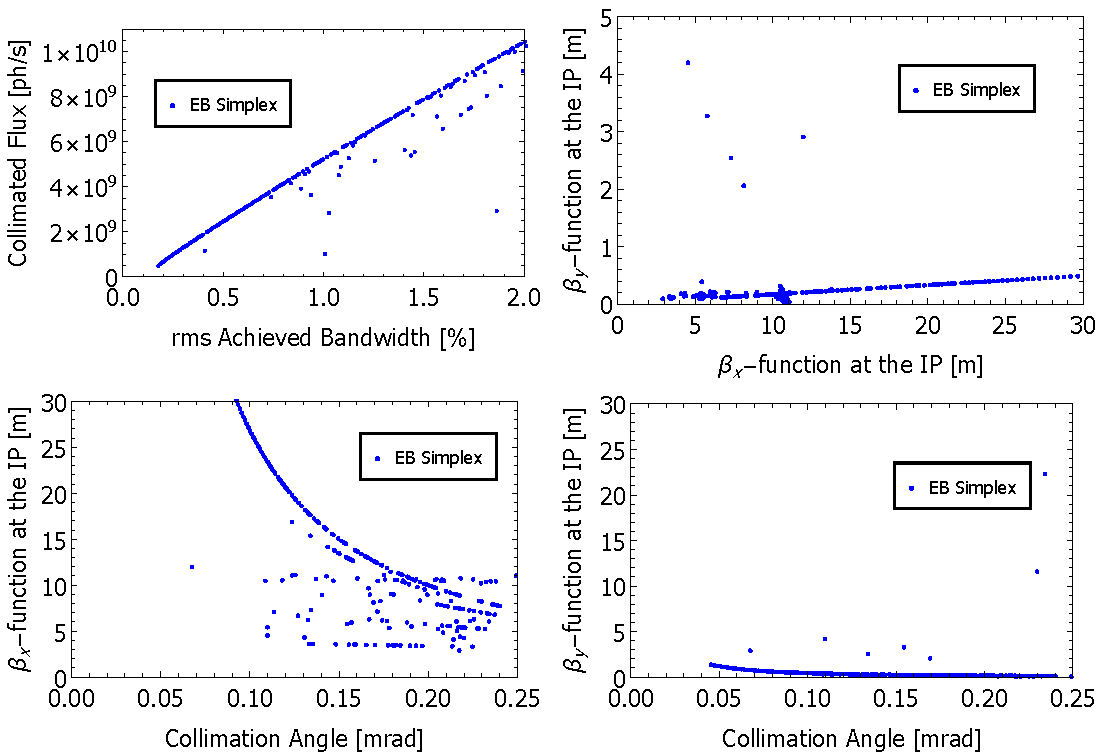
\includegraphics[width=\textwidth]{Figures/Optimisation_and_Characterisation_of_Inverse_Compton_Scattering_Sources/CaseBoptcomp.pdf}
\caption{Comparison of the two optimisation methods: Simplex NRB (blue) and GA NRB (red), for the case B parameters (see Table~\ref{tab:char_opt_electron_bunch_parameters}). Top Left: Solution space ($\mathcal{F}_{\mathrm{col}}$--$\left(\Delta E_{\gamma}/E_{\gamma}\right)_{\mathrm{rms}}$) Pareto-optimal fronts. Top Right: Parameter space ($\beta_{x}^{*}$--$\beta_{y}^{*}$) variable fronts corresponding to the Pareto-optimal fronts in solution space. Bottom Left: Parameter space ($\beta_{x}^{*}$--$\theta_{\mathrm{col}}$) variable fronts corresponding to the Pareto-optimal fronts in solution space. Bottom Right: Parameter space ($\beta_{y}^{*}$--$\theta_{\mathrm{col}}$) variable fronts corresponding to the Pareto-optimal fronts in solution space.}
\label{fig:case_B_optimisation_comparison)}
\end{figure}

The $\beta$-function at the IP parameter space ($\beta_{x}^{*}$--$\beta_{y}^{*}$) in Fig.~\ref{fig:case_B_optimisation_comparison)} shows that the solutions to the NRB optimisation are strongly biased toward a larger $\beta_{x}^{*}$ and smaller $\beta_{y}^{*}$. The tuning curves for the simplex and GA NRB optimisation methods agree well though there are some anomalous local minima points within the simplex dataset and some points are clustered around $\beta_{x}^{*} = 10$~\si{\meter}. Many local minima can be observed in the simplex NRB $\beta_{x}^{*}$--$\theta_{\mathrm{col}}$ parameter space tuning curves, however this broadly agrees with the GA NRB method. The $\beta_{y}^{*}$--$\theta_{\mathrm{col}}$ parameter space shows that $\beta_{y}^{*} < 1$~\si{\meter} are favoured past 50~\si{\micro\radian} collimation angle, though the simplex NRB method fails to define the large $\beta_{y}^{*}$-function region ($\theta_{\mathrm{col}} < 50$~\si{\micro\radian}) of the `elbow' shape plot unlike the NRB GA tuning curve optimisation. 

The case C collimated flux--\textit{rms} bandwidth tuning curves in Fig.~\ref{fig:case_C_optimisation_comparision} shows good agreement between all three methods (RB, simplex NRB, GA NRB), unlike in case A and B, because the emittance is very small ($\epsilon_{n} = 0.1$~\si{\milli\meter}--\si{\milli\radian}) and the electron bunch is short, so the angular crossing effect (Eq.~\ref{eq:angular_crossing_factor}) is minimal. Around $2.4\times 10^{8}$~ph/\si{\second} are available in a 1\% rms bandwidth. As in case B, a discrepancy is also present between the GA NRB and the simplex NRB optimisation in the narrowband region $\left(\Delta E_{\gamma}/E_{\gamma}\right)_{\mathrm{rms}} < 0.15$\% of the tuning curve. The discrepancy occurs because of a lack of individuals in the GA NRB optimisation achieving the narrowest bandwidths.       

\begin{figure}[!h]
\centering
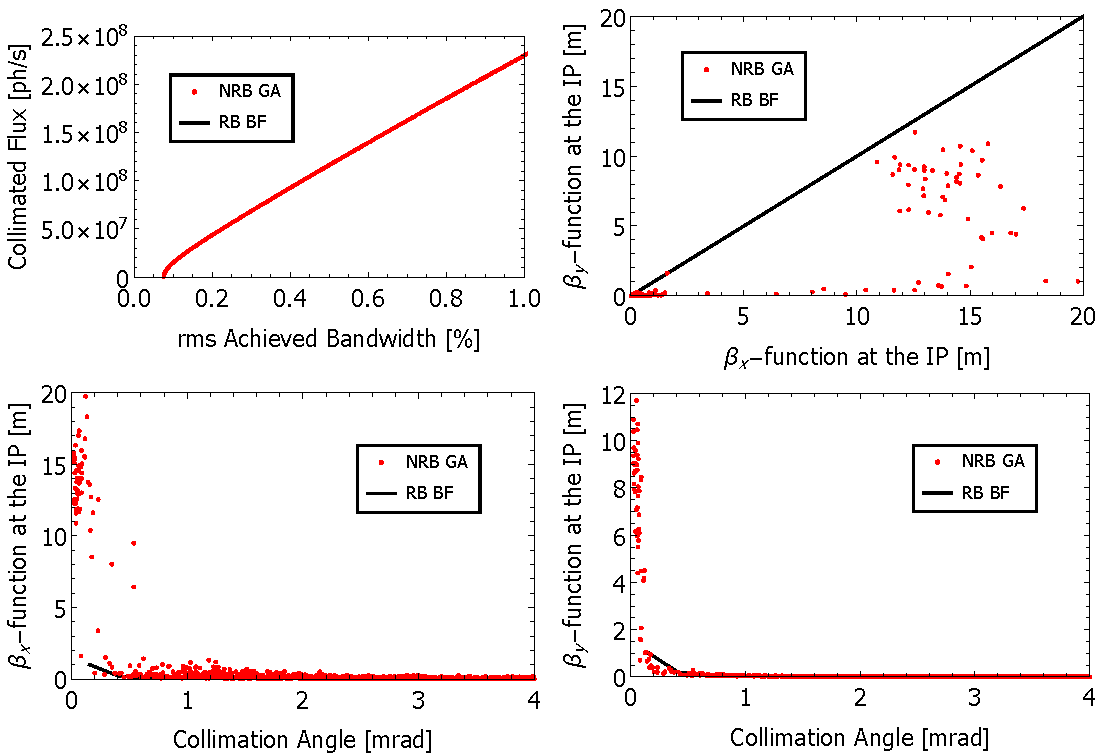
\includegraphics[width=\textwidth]{Figures/Optimisation_and_Characterisation_of_Inverse_Compton_Scattering_Sources/CaseCoptcomp.pdf}
\caption{Comparison of the three optimisation methods: RB (black), GA NRB (red) and simplex NRB (blue), for the case C parameters (see Table~\ref{tab:char_opt_electron_bunch_parameters}). Top Left: Solution space ($\mathcal{F}_{\mathrm{col}}$--$\left(\Delta E_{\gamma}/E_{\gamma}\right)_{\mathrm{rms}}$) Pareto-optimal fronts. Top Right: Parameter space ($\beta_{x}^{*}$--$\beta_{y}^{*}$) variable fronts corresponding to the Pareto-optimal fronts in solution space. Bottom Left: Parameter space ($\beta_{x}^{*}$--$\theta_{\mathrm{col}}$) variable fronts corresponding to the Pareto-optimal fronts in solution space. Bottom Right: Parameter space ($\beta_{y}^{*}$--$\theta_{\mathrm{col}}$) variable fronts corresponding to the Pareto-optimal fronts in solution space.}
\label{fig:case_C_optimisation_comparision}
\end{figure}

The $\beta_{x}^{*}$--$\beta_{y}^{*}$ parameter space tuning curve shows that the GA NRB and simplex NRB optimisations favour $\beta_{x}^{*} > \beta_{y}^{*}$, however there are some GA NRB solutions clustered around $\beta_{x}^{*} = 14$~\si{\meter}, $\beta_{y}^{*} = 8$~\si{\meter} which differ from the linear trend. The clustered points correspond to the narrowest bandwidth solutions. In the $\beta_{x/y}^{*}$--$\theta_{\mathrm{col}}$ parameter space plots the 'elbow' shapes are very severe like the  case B $\beta_{y}^{*}$--$\theta_{\mathrm{col}}$ tuning curve in Fig.~\ref{fig:case_B_optimisation_comparison)} because the emittance in the direction of the $\beta$-function is very small. The gradient of the `elbow' shape $\beta^{*}$--$\theta_{\mathrm{col}}$ plots becomes steeper with small emittance. The simplex method appears to fail to map the steep, high $\beta$-function ($\beta_{x/y}^{*} > 3$~\si{\meter}), small collimation angle ($\theta_{\mathrm{col}} < 0.3$~\si{\milli\radian}) section of the parameter space tuning curves which correspond to the narrowest bandwidth solutions. The simplex NRB method performs poorly due to the sharp gradient, which results in local minima, as small increases in the $\beta$-functions yield small reductions in the bandwidth, which slows the convergence of the simplex optimisation. Similarly the NRB GA method struggles to map the parameter space, evidenced by the reduction in Pareto-optimal individuals around $3~\si{\meter} < \beta_{x}^{*} < 10$~\si{\meter}. 

In summary, the tuning curves in Figs.~\ref{fig:case_A_optimisation_comparison}, \ref{fig:case_B_optimisation_comparison)} and \ref{fig:case_C_optimisation_comparision} show that the optimisation methods developed within this chapter (RB, simplex NRB, GA NRB) are adept at mapping out the parameter space of an ICS source. Solution space tuning curves have shown the collimated flux increases near linearly with the \text{rms} bandwidth, and that there is a low bandwidth cut-off that can not be surpassed due to the energy spread of the electron bunch and spectral bandwidth of the laser pulse. Parameter space tuning curves, which correspond to the tuning curves in collimated flux--\textit{rms} bandwidth space, such as the $\beta_{x}^{*}$--$\beta_{y}^{*}$ tuning curves have demonstrated the optimal solution is to have a non-round transverse electron bunch at the interaction point. Whilst the $\beta_{x/y}^{*}$--$\theta_{\mathrm{col}}$ parameter space tuning curves for each case have shown that the narrowest bandwith ICS source configurations involve high $\beta$-functions at the IP and small collimation angles. The trade-off between the $\beta_{x/y}^{*}$-$\theta_{\mathrm{col}}$ creates an `elbow' shaped curve in the parameter space, which has a steeper gradient with increasingly small emittance.      

\section{Summary}

Within this chapter an analytical collimated flux calculation (Eq.~\ref{eq:collimated_flux}) has been developed which is beneficial over calculations such as the formulation by Curatolo et al (Eq.~\ref{eq:curatolo_collimated_flux}) \cite{curatolo2017analytical} because it fully accounts for a crossing angle between the laser pulse and electron bunch (in both cross section and geometric luminosity reduction) as well as the hourglass effect (Eq.~\ref{eq:furman_hourglass_reduction}). The derived collimated flux formula is generalised, but excludes the energy spread of the electron bunch and laser pulse spectral bandwidth. An ICS spectrum code \textsc{ICARUS} has been developed based on the improved and corrected model by Sun et al \cite{sun2009characterizations,sun2011theoretical} accounting for recoil of the electron bunch, emittance effects, collimation, energy spread of the electron bunch, spectral bandwidth of the laser pulse and is valid in the head-on ($\phi=0$) linear ($a_{0} \ll 1$) regime. The collimated flux calculation, Curatolo et al collimated flux calculation (Eq.~\ref{eq:curatolo_collimated_flux}), \textsc{ICARUS} spectrum code and \textsc{ICCS3D} spectrum code created by Krafft et al \cite{krafft2016laser,ranjan2018simulation} have been benchmarked against each other yielding good agreement between all except the formulation by Curatolo et al \cite{curatolo2017analytical}. Agreement between these codes allowed for the spectrum of an ICS source to be quantitatively characterised by these methods, with confidence in the spectral density units. Overall, this work has allowed for better characterisation of ICS sources, which is necessary in maximising their performance.

Studies have shown that simplistic methods of ICS source IP design like transverse profile matching are sub-optimal, consequently a series of optimisations have been developed toward maximising the collimated flux within a narrow bandwidth via adjusting the electron bunch $\beta$-functions at the IP and the collimation angle. Narrow bandwidth ICS sources provide good resolution of energy dependent phenomena for experiments and high collimated flux improves the signal-to-noise ratio and data acquisition times of measurements. The optimisation of the electron bunch transverse profile and the collimation angle by the the round beam (Section~), simplex non-round beam (Section~) and genetic algorithm non-round beam methods has shown an advantage of up to $\sim 40$\% in collimated flux, and NRB optimisations have consistently out-performed RB optimisations. Two optimisation types have been developed: single point bandwidth optimisations and tuning curve optimisations. Single point optimisations allow the optimal configuration of an ICS source for a particular bandwidth to be found whereas tuning curves map the possible operational settings of an ICS source -- as is best practice for other accelerator light sources such as synchrotron light sources and free electron lasers. Tuning curve optimisations have shown there is a natural limit on the bandwidth of an ICS source because of the energy spread of the electron bunch and laser pulse spectral bandwidth, that the relationship between bandwidth and collimated flux is linear for an ICS source and that increasing the $\beta$-functions at the IP whilst minimising the collimation angle allows for the production of the narrowest bandwidth radiation. Advancements in both characterisation and optimisation enable ICS sources to be designed with higher collimated flux and narrower bandwidths, with better prediction of the spectral output. 

\end{document}